% !TeX spellcheck = en_US
\documentclass[12pt, a4paper]{article}
\usepackage{comment}
\usepackage{ragged2e}
\usepackage{amsmath}
\usepackage{xcolor}
\usepackage{multirow}
\usepackage{caption}
\usepackage{tikz}
\usepackage{booktabs}
\usepackage{tabu}
\usepackage{placeins}
\usepackage{pdflscape}
\usetikzlibrary{arrows}
\usepackage{hyperref}
\usepackage{multirow}
\usepackage{subcaption}
\usepackage{pdflscape}
\usepackage{tabularx}
\usepackage{geometry}
\usepackage{cleveref}
\usepackage{color,soul}
\usepackage{longtable}
\usepackage{rotating,tabularx,natbib,ragged2e,booktabs,caption}
%\captionsetup{font=footnotesize,labelfont=footnotesize}

\makeatletter
\newcommand*{\centerfloat}{%
  \parindent \z@
  \leftskip \z@ \@plus 1fil \@minus \textwidth
  \rightskip\leftskip
  \parfillskip \z@skip}
\makeatother



\hypersetup{
    colorlinks=true,
    linkcolor=blue,
    filecolor=blue,      
    urlcolor=blue,
    citecolor=blue
}

\usepackage{natbib}
\usepackage[title]{appendix}
\usetikzlibrary{patterns,positioning}

\tikzstyle{startstop} = [rectangle,dashed, rounded corners, minimum width=2cm, minimum height=0.75cm,text centered, draw=black, fill=red!15]

\tikzstyle{startstop1} = [rectangle, rounded corners, minimum width=2cm, minimum height=0.75cm,text centered, draw=black, fill=blue!30,pattern=dots,pattern color=blue!30]

\tikzstyle{startstop2} = [rectangle, rounded corners, minimum width=2cm, minimum height=0.75cm,text centered, draw=black, fill=yellow!30,,pattern=crosshatch,pattern color=yellow!30]

\tikzstyle{startstop3} = [rectangle , rounded corners, minimum width=0.5cm, minimum height=0.75cm,text centered,draw=black]


\tikzstyle{io} = [trapezium, trapezium left angle=70, trapezium right angle=110, minimum width=2cm, minimum height=0.75cm, text centered, draw=black, fill=blue!30]



\tikzstyle{process} = [rectangle, minimum width=2cm, minimum height=1cm, text centered, draw=black, fill=green!30]

\tikzstyle{decision} = [diamond, minimum width=0.75cm, minimum height=0.75cm, text centered, draw=black, fill=green!30]

\tikzstyle{arrow} = [thick,->,>=stealth]



\def\sym#1{\ifmmode^{#1}\else\(^{#1}\)\fi}


\renewcommand{\today}{\ifcase \month \or January\or February\or March\or %
April\or May \or June\or July\or August\or September\or October\or November\or %
December\fi, \number \year} 



\def\boxit#1{%
  \smash{\color{red}\fboxrule=1pt\relax\fboxsep=2pt\relax%
  \llap{\rlap{\fbox{\vphantom{0}\makebox[#1]{}}}~}}\ignorespaces
}


\usepackage{lipsum}

%\linespread{1.2}
\captionsetup[subtable]{labelformat=empty}
\title{{Connected Stocks via Business Groups: Evidence from an Emerging Market}}
\author{{S.M. Aghajanzadeh\sym{*} \qquad M. Heidari\sym{*} \qquad M. Mohseni\sym{*} }\\
{\sym{*} \footnotesize  Tehran Institute for Advanced Studies, Khatam University, Tehran, Iran}
}




\begin{document}
\maketitle



\begin{abstract}

 We link stocks through direct and indirect common owners, showing that common ownership and belonging to a business group (indirect common owner) affect the stock price co-movement. Our analysis is based on the daily ownership of block-holders on the Tehran Stock Exchange. We show that belonging to a business group has a higher effect than having a common owner, which influenced only movement within business groups. In addition, simultaneous trades in the same direction explain comovement in business groups.

\end{abstract}






\section{Introduction}
%%%%%%%%%%%%%%%%%%%%%%%%%%%%%%%%%%

Existing literature has well established that stocks comove with each other. One collection of studies suggests that commonality in fundamental values generates comovement in stock return. This suggestion is derived from economics without frictions and rational investors. For example, \cite{shiller1989comovements} provides evidence that the comovement of real dividends could be accounted for the comovement in real stock prices.
	Although, in recent years, it has been recognized that the comovement rises from non-fundamental sources. {\cite{barberis2003style} and \cite{barberis2005comovement}} provided theoretical models for predicting a comovement between fundamentally unrelated companies. Trying to explain factors affecting comovement, {\cite{AntonPolk}} examined the effect of common ownership\footnote{The common ownership concept has been observed in financial literature in recent years. There has been a surge in the popularity of index investing in the United States, which has led to an increase in common ownership. 
			For instance, \cite{azar2018anticompetitive} claims that an increase in mutual ownership in airline companies leads to less competitive ticket pricing. However, this subject is controversial, and many papers discuss whether mutual ownership affects companies' behavior.
			For example, \cite{lewellen2021does} realized that in previous investigations, other effective factors have wrongly been replaced by the mutual ownership effect.
		} on comovement\footnote{	The followings are some of the other sources of comovement. Index inclusion ({\cite{barberis2005comovement}}), investors' attention to the companies ({\cite{wu2014investor}}), Investment banks' underwriting ({\cite{grullon2014comovement}}), correlated beliefs ({\cite{david2016correlated}}), shareholders' coordination ({\cite{pantzalis2017shareholder}}), and preference for companies' dividends ({\cite{HAMEED2019103}}) are among contributing factors to comovement that have been identified by researchers.}. This paper uses mutual funds' ownership and suggests that comovement increases by increasing common ownership. Also, it is shown in the paper that the comovement increases when there is a significant net flow, either in or out-flow in the months.
	
	Subsequently, according to {\cite{Liquidity2016}} companies show comovement considering their owners' correlation in their liquidity needs. The author also adds that companies with higher mutual fund ownership have a more liquidity correlation than others. This paper contends that in order for companies to have comovement, there is no need for common ownership. Plus, common ownership can explain companies'  liquidity correlation. 
	
While most of the prior investigations on factors affecting common-ownership have focused on the fund, the role of the block-holders as one of the most important factors in firms' governance has remained a black box\footnote{A long literature surveyed by \cite{holderness2003survey}, \cite{edmans2014blockholders}, and \cite{edmans2017blockholders} considers the potential role of blockholders in firm governance}. Funds behave differently due to their needs and the fact that they are intermediates, making it difficult to generalize these results to other types of ownership. \cite{edmans2014 governance} provide a theoretical model to investigate the implications of common ownership of block holders for corporate governance and asset pricing. Nevertheless, in Iran, the block holders' daily ownership data, including mutual fund ownership, is publicly accessible. So research through this data can show whether common ownership other than mutual fund ownership can lead to comovement or not. Following \cite{AntonPolk}, we are the first study that uses block-holder ownership to investigate the relationship between common ownership and comovement.
	
	

		
Despite the presence of the business group in both emerging economies, e.g., Brazil, Chile, China, India, Indonesia, South Korea, and developed countries, e.g., Italy, Sweden, (\cite{khanna2007business}), there is no evidence on whether being at the same business group can lead to the comovement. Business groups consist of legally independent firms operating across diverse industries different from commonly held firms. Although researchers have identified comovement among stock
returns,  to the best of our knowledge, we are the first comprehensive study about the different roles of the business groups and common ownership on comovement. 


%%%%%%%%%%%%%%%%%%%%%%%%%%%%%%%%%%
%%%%%%%%%%%%%%%%%%%%%%%%%%%%%


%	
%	Both {\cite{cho2015stock} and \cite{kim2015stock}} studied the South Korean market and suggested two different sources for the comovement in business groups. The first paper attributed comovement to the companies' fundamentals. However, the second paper presents that the investors' category/habitat behavior is responsible for comovement.
%	
%	In this paper, we consider the comovement of the companies in business groups. Best of our knowledge, it is the first study that compares direct and indirect common ownership.
%	A modified measurement is introduced in this paper to calculate the common ownership of the companies. 


We hypothesize that stocks with a high level of common ownership and the same ultimate owner exhibit strong comovement. In fact, when we talk about the presence of two stocks in the same business group, we talk about a high level of invisible common ownership between two stocks that we cannot measure by common ownership measurements. 

%% Result
We test this hypothesis using \cite{AntonPolk} methodology and realize that common ownership is crucial for predicting the comovement. Business groups play a more critical role in predicting the correlation of companies' returns than common ownership, with a coefficient about six times as large as the common ownership coefficient. Furthermore, We show that common ownership can predict comovement only inside the business groups.



We extend our analysis to validate the prominence of business groups. First, we find that the average of common ownership is five times larger for the firms in the business group. So, we restrict the study to the high level of common ownership to distinguish the effect of common ownership and business groups. In this subsample, like the mentioned ones, business groups significantly impact firms' comovement. Second, if business groups affect comovement, there is no need to restrict our investigation to firms with common owners, and also this would affect all the firms in the market. To address these concerns and distinguish the impact of common ownership and business group, we extend our investigation to all the firms in the market and show that the business group can increase firms' comovement. 
	
	Finally, we show that correlated trade in business groups is the channel of comovement. We provide evidence that the volume and direction of trades in business groups are related, and firms in the business groups with higher relation in trade have a higher level of comovement.
	
	
	%  The business groups might not have as much influence as the market has on many companies' turnover fluctuations. However, it is influential.
	% The companies' presence in business groups can explain the correlation in turnover. 
	% We extracted both yearly companies' turnover average and monthly market turnover from monthly companies' turnover. Then we realized that there is less monthly residual dispersion in business
	% groups analyzing the deduced data.
	% More comovement is detected for groups with less dispersion.
	% 
	% Institutional imbalance:
	% Institutional imbalance dispersion must be low for these companies.
	% In general, the imbalance dispersion average in business groups is less than companies that are not included in the groups.
	% A more precise study illustrated that determining business groups with low dispersion, we expect the comovement to increase.
	% In low dispersion groups, the comovement increases with either a decrease in dispersion or with higher common ownership.
	% We searched for fundamental factors, too. But they had no impact on price comovements.-
	

%%%%%%%%%%%%%%%%%%%%%%%%%%%%%
%\section{Introduction}
در سال های اخیر با
\begin{itemize}
\item
هم حرکتی مورد توجه تحلیلگران بازار و محققان قرار گرفته است
\item
بعد از بحران مالی سال 2007 مدل های برآورد ریسک اهمیت پیدا کرده است
\item
در این مدل ها هم بستگی قیمت دارایی ها نقش تاثیرگذاری در برآورد ریسک دارد
\item
پاسخ سنتی به دلیل هم حرکتی بازده شرکت ها عوامل بنیادی دو شرکت بوده است  برای مثال 
 \lr{\cite{shiller1989comovements}}
 \item 
 ولی در سال های اخیر نشان داده شده است که هم حرکتی می تواند از عواملی غیر بنیادی به وجود بیاید. 
 \item
 مدل های تئوری برای  هم حرکتی میان بازده شرکت های غیر مرتبط از لحاظ بنیادی
 \lr{\cite{barberis2003style},\cite{barberis2005comovement}}
 \item
 معرفی عوامل دیگر برای هم حرکتی قیمت شرکت ها
 \begin{itemize}
 \item 
 عضو بودن شرکت ها در شاخص
  \lr{S\&P500} [\lr{\cite{barberis2005comovement}}]
      \item
      توجه سرمایه گذاران به شرکت ها
      [\lr{\cite{wu2014investor}}]  
        \item 
      پذیره نویسی توسط بانک سرمایه گذاری 
      (\lr{investment bank})
      
      [\lr{\cite{grullon2014comovement}}]  
      \item
      باور های یکسان و مرتبط
      [\lr{\cite{david2016correlated}}] 
         \item
         هم زمان بودن نیاز های نقدینگی سهامداران شرکت ها
         [\lr{\cite{pantzalis2017shareholder}}]  
            \item
         پرداخت سود تقسیمی توسط شرکت ها
         [\lr{\cite{HAMEED2019103}}]  
 \end{itemize}



\end{itemize}

\begin{itemize}
\item 
از طرف دیگر در سال های اخیر مسئله مالکیت مشترک ادبیات مالی مورد توجه قرار گرفته است
\footnote{
	با توجه به افزایش صندوق های سرمایه گذاری  دنبال کننده شاخص در آمریکا، مسئله مالکیت مشترک در میان شرکت های آمریکا افزایش داشته است و این امر سبب شده است که در ادبیات مسئله بررسی مالکیت مشترک و عملکرد شرکت ها و همچنین رفتار بازده ای شرکت ها مورد توجه قرار گیرد. 
	برای مثال 
	\lr{\cite{azar2018anticompetitive}}
	با افزایش مالکیت مشترک میان شرکت های هواپیمایی رقابت قیمتی شرکت ها کاهش پیدا می کند.  اما در این رابطه بحث و گفت و گو همچنان ادامه دارد و مقالات زیادی در رد و تایید اثر مالکیت مشترک بر روی رفتار شرکت ها وجود دارد. برای مثال مقاله
	\lr{\cite{lewellen2021does}}
	مقالات سال های گذشته را بررسی کرده است و یافته است که در بررسی های گذشته، اثر دیگر فاکتور های تاثیر گذار به اشتباه به مالکیت مشترک مرتبط شده است.
}
 و
\lr{\cite{AntonPolk}}
اثر مالکیت مشترک را بر هم حرکتی را بررسی کرده است.  

\begin{itemize}
\item \lr{\cite{AntonPolk}}
\begin{itemize}
\item
یافته است که با افزایش مالکیت مشترک هم حرکتی شرکت ها افزایش پیدا می کند. 
%\item
%علاوه بر این با توجه به دسترسی به داده های مالکیت صندوق های سرمایه گذاری مقاله نشان داده است که هم حرکتی شرکت ها هنگامی که جریان خروجی و ورودی قوی ای در صندوق ها وجود داشته باشد افزایش پیدا می کند. 
\item
این مقاله بررسی خود را محدود به صندوق های سرمایه گذاری فعال 
(\lr{Active mutual funds}) 
و شرکت های بزرگ (ارزش بازاری بالاتر از میانه ارزش شرکت ها) محدود کرده است.
\end{itemize}
\end{itemize}
\item
در ادامه 
\lr{\cite{Liquidity2016}}
نشان داده است که شرکت ها با توجه به هم بستگی نیاز های نقدینگی مالکان خود، با یکدیگر هم حرکتی نشان می دهند
\begin{itemize}
\item \lr{\cite{Liquidity2016}}:
\begin{itemize} 
\item
 نشان می دهد که شرکت های دارای سطح بالایی از مالکیت صندوق های سرمایه گذاری همراهی نقدشوندگی بالاتری نسبت به بقیه شرکت ها دارند.
 \item
 نشان می دهد که برای هم حرکتی قیمت شرکت ها نیاز به مالکیت مشترک نیست
 \item
 همچنین نشان می دهد که مالکیت مشترک می تواند هم بستگی در نقد شوندگی سهام شرکت را توضیح دهد
\end{itemize}

\item
نتایج به دست آمده در پژوهش های قبلی با استفاده از داده های مالکیت صندوق های سرمایه گذاری بدست آمده است
\item
در نتیجه نتایج بدست آمده محدود به این نوع مالکیت می باشد
\item
در صورتی که این نوع به خصوص مالکیت با توجه به نیاز ها و واسطه بودن، رفتار های به خصوصی انجام می دهند
\footnote{\lr{\cite{coval2007asset}} 
	نشان داده است که جریان ورود و خروج مالی صندوق ها می تواند سبب ایجاد فشار قیمتی بر سهام شرکت ها شود و قیمت شرکت ها رو تحت تاثیر قرار دهد و این مسئله با موصوع مالکیت مشترک که می تواند سبب تغییر رفتار مدیران شرکت شود می تواند متفاوت باشد.}

\end{itemize}

\item 
از طرفی دیگر 
یکی دیگر از ویژگی های بازار سرمایه ایران وجود گروه های کسب و کار است. گروه های کسب و کار حدود 85\% از ارزش بازار ایران را در اختیار دارند.
\begin{itemize}
	\item
	گروه های کسب و کار پدیده مهمی هستند در کشور های در حال توسعه یافته و در حال توسعه وجود دارند.
	\item
	هم حرکتی شرکت ها را در گروه های کسب و کار بررسی می کنیم
	\item
	دو مقاله در ادبیات به این موضوع پرداخته اند و هم حرکتی قیمت شرکت ها در گروه های کسب و کار را بررسی کرده اند
	\item
	هم حرکتی قیمت شرکت ها در گروه های کسب و کار تایید شده است ولی کانال این هم حرکتی مشخص نشده است
	\begin{itemize}
		\item \lr{\cite{cho2015stock},\cite{kim2015stock}}:
		\begin{itemize}
			دو پاسخ متفاوت به دلایل هم حرکتی شرکت ها در گروه های کسب و کار داده اند. هر دو گروه های کسب و کار موجود در بازار کره جنوبی را بررسی کرده اند و مقاله اول عوامل بنیادی مرتبط شرکت ها در گروه های کسب و کار را به عنوان دلیل هم حرکتی شرکت ها معرفی کرده است ولی مقاله دوم دسته بندی شرکت های عضو گروه را به عنوان دلیل هم حرکتی بیان کرده است. 
		\end{itemize}
		
	\end{itemize}

\end{itemize}
\item
در این بستر می توان اثر مالکیت مشترک مستقیم و غیر مستقیم را بررسی کرد
\end{itemize}

%%%% Our work
\begin{itemize}
\item 
در این پژوهش 
\item
اولین بررسی هم حرکتی ناشی از مالکیت مشترک صرف نظر از اینکه مالک شرکت صندوق سرمایه گذاری بوده باشد

\item 
در ایران داده های مالکیت های بالای یک درصد به صورت روزانه وجود دارد که محدود به مالکیت صندوق های سرمایه گذاری نیست.
\item
می توان به این سوال پاسخ داد که مالکیت مشترک فارغ از نوع مالکان سبب هم حرکتی می شود و یا خیر
\end{itemize}

%با توجه به محدودیت های دیتای موجود در آمریکا و  تنها موجود بودن داده های مالکیت های صندوق های سرمایه گذاری، بخشی از بررسی های این حوزه محدود به اثر مالکیت صندوق های سرمایه گذاری بر شرکت ها می باشد. برای مثال مقاله 
%\lr{\cite{coval2007asset}} 
%نشان داده است که جریان ورود و خروج مالی صندوق ها می تواند سبب ایجاد فشار قیمتی بر سهام شرکت ها شود و قیمت شرکت ها رو تحت تاثیر قرار دهد و این مسئله با موصوع مالکیت مشترک که می تواند سبب تغییر رفتار مدیران شرکت شود می تواند متفاوت باشد.


%در ایران با توجه به دسترسی به داده های مالکیت های بالای یک درصد شرکت ها به صورت روزانه، می توان با دقتی بالاتر و مشخص تر اثر مالکیت مشترک را بر روی شرکت های ثبت شده در بازار بورس مشخص کرد.  از طرف دیگر یکی دیگر از ویژگی های بازار سرمایه ایران وجود گروه های کسب و کار است. گروه های کسب و کار حدود 85\% از ارزش بازار ایران را در اختیار دارند.  در بازار های در حال توسعه در اکثر نقاط دنیا و حتی بعضی از کشرو های توسعه یافته نیز گروه های کسب و کار وجود دارند. گروه های کسب و کار مجموعه از شرکت های مرتبط با یکدیگر هستند که دارای مالک نهایی یکسان می باشند. در ادبیات موارد متعددی در رابطه با تاثیر گروه های کسب و کار بر روی شرکت ها معرفی  شده است. در رابطه با بررسی هم حرکتی در شرکت ها دو مقاله 
%\lr{\cite{cho2015stock},\cite{kim2015stock}}
%این موضوع را بررسی کرده اند و دو پاسخ متفاوت به دلایل هم حرکتی شرکت ها در گروه های کسب و کار داده اندد. هر دو گروه های کسب و کار موجود در بازار کره جنوبی را بررسی کرده اند و مقاله اول مسائل بنیادی مرتبط شرکت ها در گروه های کسب و کار را به عنوان دلیل هم حرکتی شرکت ها معرفی کرده است ولی مقاله دوم دسته بندی شرکت های عضو گروه را به عنوان دلیل هم حرکتی بیان کرده است.


\begin{itemize}
\item
در این مقاله سعی شده است تا هم حرکتی میان شرکت های درون گروه های کسب و کار بررسی شود.

\item 
و برای اولین میان مالکیت مشترک مستفیم و مالکیت مشترک غیر مستقیم مقایسه انجام شود

\end{itemize}
 
 
 \begin{itemize}
 \item
برای محاسبه مالکیت مشترک میان شرکت ها از ملاکی اصلاح شده استفاده کرده ایم که در این پژوهش معرفی کرده ایم

 \end{itemize}


\begin{itemize}
\item
مالکیت مشترک برای پیش بینی هم حرکتی قیمت شرکت ها اهمیت دارد
\item 
گروه های کسب و کار برای پیش بینی هم حرکتی قیمت شرکت ها اهمیت دارد
\item
اهمیت گروه های کسب و کار برای پیش بینی هم حرکتی قیمت شرکت ها بیشتر از مالکیت مشترک است
\item
 در گروه های کسب و کار، مالکیت مشترک سبب افزایش هم حرکتی قیمت می شود ولی در خارج از گروه های کسب و کار اهمیت ندارد
\end{itemize}



\begin{itemize}
\item 
انواع بررسی ها برای تایید اهمیت گروه های کسب و کار انجام شده است 
\begin{itemize}

\item
فقط جفت  های د ارای مالکیت بالا را بررسی کردیم
\begin{itemize}
\item 
در این زیر مجموعه هم گروه های کسب و کار بیشترین تاثیر را دارند 
\item
مالکیت مشترک صرفا در گروه های کسب و کار اهمیت دارند.

\end{itemize}
\item
بررسی ها محدود به جفت های دارای مالک مشترک بوده است:
\begin{itemize}
\item
بررسی اثر گروه کسب و کار نیاز به مالکیت مشترک ندارد
\item
اثر گروه کسب و کار و مالکیت مشترک را نمی توان جدا کرد
\item 
همه ی جفت های بازار را ساختیم و اهمیت گروه ها کسب و کار نسبت به مالکیت مشترک مستقیم تایید شده است.
%\begin{itemize}
%\item
%نتایج اولیه تایید شد
%\item 
%جفت های حاضر در گروه های کسب و کار سطح مالکیت مشترک اهمیت ندارد و صرفا سطح بالایی از مالکیت مشترک اهمیت دارد
%\item
%برای جفت های بیرون یک گروه کسب وکار، سطح مالکیت در واقع وجود مالکیت مشترک اهمیت دارد و نه مقدار قابل توجه آن
%\item
%مالکیت مشترک خارج از گروه های کسب و کار نیز اهمیت دارد
%\item
%تاثیر یکسان بودن گروه های کسب و کار بیشتر است
%\end{itemize}
\end{itemize}

\end{itemize}


	\item
کانال تاثیر: معامله هم زمان شرکت ها با یکدیگر در گروه های کسب و کار
\begin{itemize}

	\item
	از دو پراکسی برای بررسی اثر معاملات هم زمان در گروه های کسب و کار 
	\item
	\lr{turnover} 
	و ناترازی خرید و فروش حقوقی استفاده کرده ایم
	\item
	پراکسی اول معاملات هم زمان را تایید می کند
	\item
	پراکسی دوم هم جهتی معاملات را تایید می کند
	%\begin{itemize}
	%\item
	%\lr{turnover}
	%\begin{itemize}
	%\item
	%بخش قابل توجهی از تغییرات 
	%\lr{turnover}
	%شرکت ها علاوه بر بازار از گروه های کسب و کار ناشی می شود
	%\item
	%حضور شرکت ها در گروه های کسی و کار می تواند هم بستگی 
	%\lr{turnover}
	%را توضیح دهد.
	%\item
	%از 
	%\lr{turnover}
	%ماهانه شرکت ها 
	%میانگین 
	%\lr{turnover}
	%سالانه شرکت و 
	%\lr{turnover}
	%ماهانه بازار را خارج کردیم و بررسی کردیم درگروه های کسب و کار میزان پراکندگی باقی مانده ماهانه کمتر است
	%\item
	%برای گروه های با پراکندگی کمتر هم حرکتی بیشتر است
	%
	%% گروه های کسب و کار بزرگ
	%% \begin{itemize}
		%% 	\item 
		%% 	اگر معامله گران شرکت های در یک گروه کسب و کار را در یک دسته قرار می دهند نیاز است تا اعضای گروه های بزرگ هم حرکتی بیشتری داشته باشند
		%% 	\item
		%% 	علاوه بر مورد فوق باید رابطه هم بستگی 
		%% 	\lr{turnover}
		%% 	و هم حرکتی بازده نیز مثبت باشد. 
		%% 	
		%% 		\item 
		%% 		شرکت های عضو گروه کسب و کار به همراه یکدیگر معامله بشوند
		%% 		
		%% 	
		%% \item
		%% بررسی کردیم و نتایج نشان داد که شرکت های در گروه بزرگ هم حرکتی بیشتری دارند و علاوه بر این تاثیر هم حرکتی در 
		%% \lr{turnover}
		%% نیز در گروه های بزرگ از دیگر گروه ها بیشتر است.
		%% \end{itemize}
	%\end{itemize}
	%\item 
	%ناترازی خرید حقوقی
	%\begin{itemize}
	\item
	پراکندگی ناترازی خرید و فروش حقوقی در این شرکت ها باید کم باشد
	\item 
	به صورت کلی در گروه های کسب و کار میانگین پراکندگی شاخص ناترازی کمتر از شرکت های بیرون گروه است
	\item
	بررسی دقیق تر نشان داد با مشخص کردن گروه های کسب و کار دارای پراکندگی کم انتظار داریم با کاهش پراکندگی، هم حرکتی افزایش پیدا کند
	\item
	در گروه های با پراکندگی کم، هم حرکتی شرکت ها افزایش پیدا می کند و با افزایش مالکیت مشترک نیز هم حرکتی افزایش پیدا می کند
	
	\item
	کانال عوامل بنیادی را بررسی کردیم ولی تاثیری بر هم حرکتی قیمت ها یافت نشد
	
\end{itemize}



\end{itemize}







% !TeX spellcheck = <none>

\section{{Data and Methodology}}



\subsection{{Data and Sample}}



Our data have several unique features which distinguish our paper from the existing literature. Stock ownership data for Iranian public firms is available with daily frequency reported at the end of each trading day. This data includes all blockholders, defined as having at least one percent of the outstanding shares in a firm for all investor types- institutional as well as individuals- and is automatically reported by a central authority named Tehran Securities Exchange Technology Management Corporation (TSETMC), which is a subsidiary of Tehran Stock Exchange. This eliminates potential issues in self-reported data (such as those existing in US institutional holding data, known as 13F filings). In order to put together our dataset, we compile daily stock ownership tables (available in separate tables for each firm), which are publicly available starting from 2010.

We use data on business groups, defined as a group of listed firms with interconnected ownership structures controlled by an ultimate owner. Business groups are a common organizational structure in corporate ownership in Iran as well as many other parts of the world. Two-thirds of Iranian public firms are part of complex interlinked ownership networks, each governed by an ultimate owner, which sits at the top of a multi-layer pyramid ownership structure ({\cite{Aliabadi2022}}). Unlike countries like South Korea, Japan, and India that formally announce business groups, we do not have officially-defined business groups in Iran. We use data provided by {\cite{Aliabadi2022}} which builds a comprehensive dataset of all Iranian business groups. Using either of the two different methodologies, one introduced by \cite{almeida2011structure} with a 40\% threshold for control rights, and the other by \cite{aminadav2011rebuilding} which is based on Shapley-Shubik index (\cite{shapley1954method}) generates the same business group definitions in Iranian public sector({\cite{Aliabadi2022}}).\footnote{For further discussion see appendix \ref{BGDef}} Our business group data covers the period 2015-2020.  



	We also gather stock returns, trading volume, firm-level trading data, and accounting information from Codal (equivalent to SEC's EDGAR) \footnote{\href{http://www.codal.ir}{www.codal.ir}}
and TSETMC's website\footnote{\href{http://www.tsetmc.com}{www.tsetmc.com}}. We exclude ETFs. The final sample used in our empirical analysis spans from 2015 to 2020 (1393/01-1398/12 Persian calendar). 



Panel \subref{t2-1} table \ref{st1} reports summary statistics for ownership and business groups data. An average firm in our sample has six blockholders holding 75 percent of shares in aggregate. More than two-thirds of our sample firms are part of a business group. There are around 40 business groups, each consisting of, on average, seven firms.






\subsection{{Pair composition} }

	If any two firms have at least one common blockholder, we consider them a commonly held firm pair. By this definition, there are 17522  unique pairs in our entire sample period, which is 20\%of all possible pairs ($\frac{554*553}{2} = 153181$). Firm pairs in our sample have on average 1.2common owners. 
	
	An important feature of common ownership in the Iranian public sector is that business groups are the main driver of common ownership, in contrast to US data in which the rise in common ownership is generally attributed to passively managed funds such as index funds. The asset management industry, especially in the form of mutual funds or ETFs, is generally a young but growing industry in Iran and does not have a large presence in firms' ownership structures. We, therefore, also identify pairs based on whether the two firms belong to the same business groups. 
		
		If both firms in a pair belong to the same ultimate owner, we identify them as being in the same business group. The two firms in a pair could also belong to different business groups or not be part of any business groups. Figure \ref{g2-1} illustrates all possibilities based on whether firm pairs belong to the same, different, or any business groups. In about one-third of our pairs, neither of the two firms belong to any business group, while in about 10 percent of our pairs, firms are part of the same business group. Panel \subref{t2-2} of table \ref{st1} reports summary statistics for firm pairs.
	
	\captionsetup[subfigure]{labelformat=parens,font=footnotesize}
			\renewcommand{\thesubfigure}{\Alph{subfigure}}	
	\begin{figure}[htbp]
		\centering
		\caption{ Firm pairs and business groups}
		\label{g2-1}
		\normalcolor
	\bigskip
		\begin{subfigure}[t]{.6\linewidth}
			\centering
			\tiny
			\resizebox{1\textwidth}{!}{
				
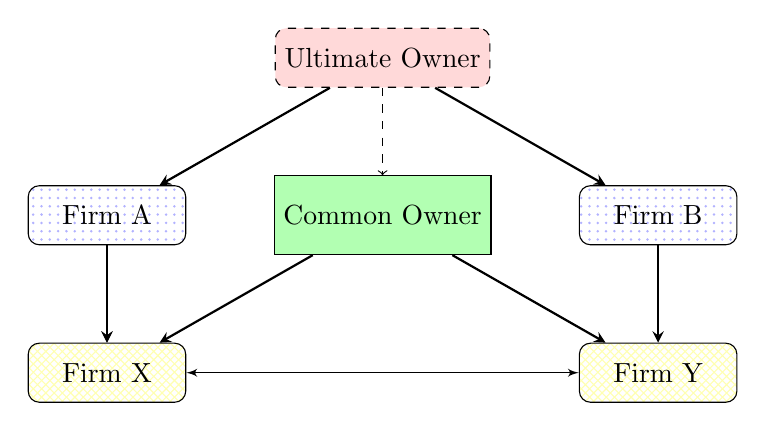
\begin{tikzpicture}[node distance=2cm]


\node (start) [startstop] {\normalsize Ultimate Owner};



\node (end) [startstop1,below of = start , yshift=0cm , xshift=-3.5cm ] {\normalsize $ \text{Firm A} $};
\node (end2) [startstop1,below of = start , yshift=0cm , xshift=3.5cm ] {\normalsize $ \text{Firm B} $};



\node (sur) [startstop2 ,below of = end ,yshift=0cm,xshift=0cm] {\normalsize $ \text{Firm X} $};


\node (sur2) [startstop2 ,below of = end2 ,yshift=0cm,xshift=0cm] {\normalsize $ \text{Firm Y} $};


\node (CH) [process, below of = start ,xshift=0] {\normalsize Common Owner};


\draw [arrow] (start) --(end);
\draw [arrow] (end) --(sur);

\draw [arrow] (start) --(end2);

\draw [arrow] (end) --(sur);
\draw [arrow] (end2) -- (sur2);


\draw [arrow] (CH) -- (sur);
\draw [arrow] (CH) -- (sur2);
\draw [dashed ,->] (start) --(CH);

\draw [latex'-latex'] (sur) to [bend right =0]  node[sloped, anchor=center, below] {} (sur2);


\end{tikzpicture}

			}
			\caption{ Pair in the same business group}
		\end{subfigure}

		\begin{subfigure}[t]{.65\linewidth}
			\centering
			\tiny
			\resizebox{1\textwidth}{!}{
						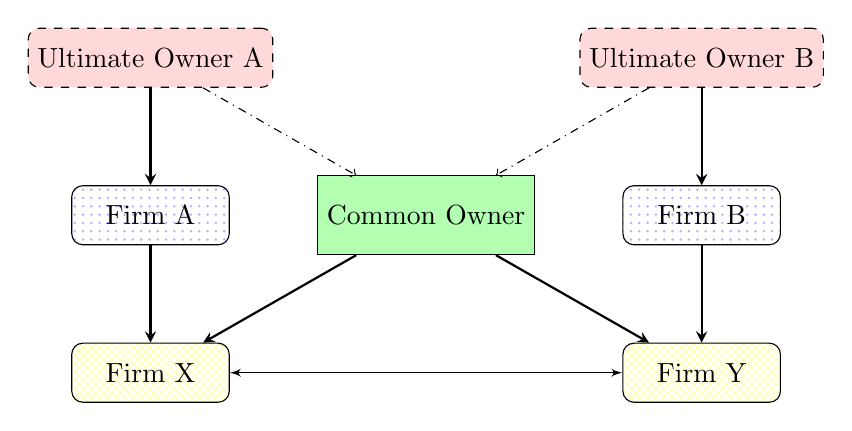
\begin{tikzpicture}[node distance=2cm]
					
					
					\node (start) [startstop] { \normalsize$ \text{Ultimate Owner A} $};
					\node (start2) [startstop,right of = start,xshift=5cm] {\normalsize$ \text{Ultimate Owner B} $};
					
					
					\node (CH) [process, below of = start2,xshift=-3.5cm] {\normalsize Common Owner};
					
					\node (end) [startstop1,below of = start ] {\normalsize $ \text{Firm A} $};
					
					\node (end2) [startstop1,below of = start2 ,yshift=0cm,xshift=0cm] {\normalsize $ \text{Firm B} $};
					
					\node (sur) [startstop2 ,below of = end ,yshift=0cm,xshift=0cm] {\normalsize $ \text{Firm X} $};
					
					\node (sur2) [startstop2,below of = end2 ,yshift=0cm,xshift=0cm] {\normalsize $ \text{Firm Y} $};
					
					
					
					\draw [arrow] (start) --(end);
					\draw [arrow] (start2) -- (end2);
					
					\draw [arrow] (end) --(sur);
					\draw [arrow] (end2) -- (sur2);
					
					\draw [dash dot,->] (start) -- (CH);
					\draw [dash dot,->] (start2) -- (CH);
					
					\draw [arrow] (CH) -- (sur);
					\draw [arrow] (CH) -- (sur2);
					
					\draw [latex'-latex'] (sur) to [bend right =0]  node[sloped, anchor=center, below] {} (sur2);
					
					
				\end{tikzpicture}
		
			}   
			\caption{ Pair in two distinct business group}
		\end{subfigure}
			\bigskip
		\begin{subfigure}[t]{1\linewidth}
			
			\resizebox{0.49\textwidth}{!}{
			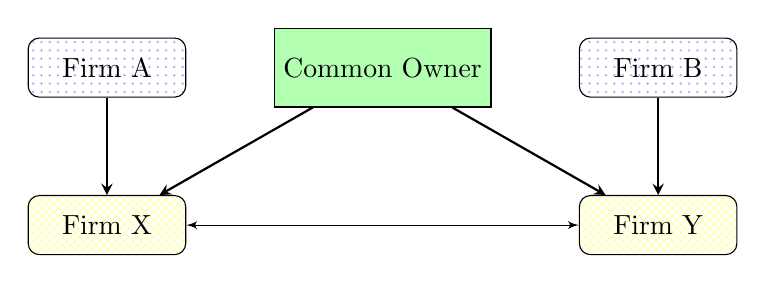
\begin{tikzpicture}[node distance=2cm]
					
					
					
					\node (CH) [process,yshift = -2cm ,xshift=3.5cm] {Common Owner};
					
					\node (end) [startstop1,left of = CH ,xshift=-1.5cm ] {$ \text{Firm A} $};
					
					\node (end2) [startstop1,right of = CH ,yshift=0cm,xshift=1.5cm] {$ \text{Firm B} $};
					
					\node (sur) [startstop2 ,below of = end ,yshift=0cm,xshift=0cm] {$ \text{Firm X} $};
					
					\node (sur2) [startstop2,below of = end2 ,yshift=0cm,xshift=0cm] {$ \text{Firm Y} $};
					
					
					\draw [arrow] (end) --(sur);
					\draw [arrow] (end2) -- (sur2);
					
					
					\draw [arrow] (CH) -- (sur);
					\draw [arrow] (CH) -- (sur2);
					
					\draw [latex'-latex'] (sur) to [bend right =0]  node[sloped, anchor=center, below] {} (sur2);
					
					
				\end{tikzpicture}
		
			}   
			\hfill
			\resizebox{0.49\textwidth}{!}{
						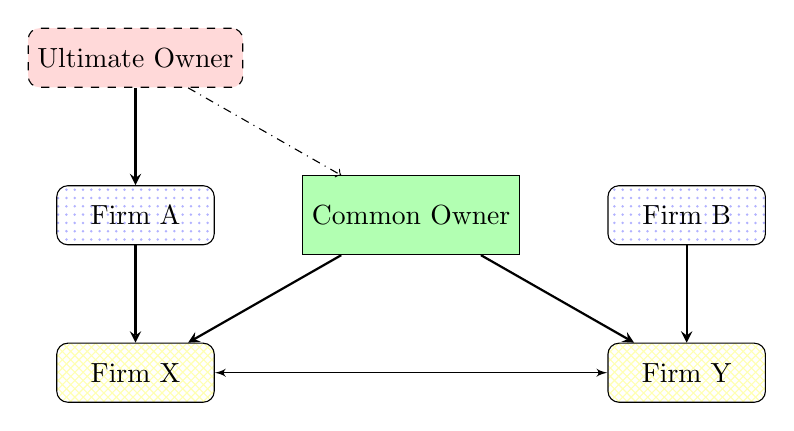
\begin{tikzpicture}[node distance=2cm]
					
					
					\node (start) [startstop] { $ \text{Ultimate Owner} $};
					
					
					\node (CH) [process, below of = start,xshift=3.5cm] {Common Owner};
					
					\node (end) [startstop1,below of = start ] {$ \text{Firm A} $};
					
					\node (end2) [startstop1,right of = CH ,yshift=0cm,xshift=1.5cm] {$ \text{Firm B} $};
					
					\node (sur) [startstop2 ,below of = end ,yshift=0cm,xshift=0cm] {$ \text{Firm X} $};
					
					\node (sur2) [startstop2,below of = end2 ,yshift=0cm,xshift=0cm] {$ \text{Firm Y} $};
					
					
					
					\draw [arrow] (start) --(end);
					
					\draw [arrow] (end) --(sur);
					\draw [arrow] (end2) -- (sur2);
					
					\draw [dash dot,->] (start) -- (CH);
					
					\draw [arrow] (CH) -- (sur);
					\draw [arrow] (CH) -- (sur2);
					
					\draw [latex'-latex'] (sur) to [bend right =0]  node[sloped, anchor=center, below] {} (sur2);
					
					
				\end{tikzpicture}
		
				}
			\caption{ Pair not in the business group}
		\end{subfigure}
			
		
		
	\end{figure}  
	
	
	\captionsetup[subfigure]{labelformat=empty}
	
\DeclareRobustCommand{\myname}{17522}


	
				
		\captionsetup[subtable]{labelformat=parens}
			\renewcommand{\thesubtable}{\Alph{subtable}}
			 \begin{table}[htbp]
			 \caption{ Summary Statistics \\ \small
			 This table reports summary statistics of ownership features for all TSE stocks from 2015 to 2020. Panel \subref{t2-1} lists the total number of firms and Business groups and other features as of the year end for each of the years in our sample. Panel \subref{t2-2} reports summary statistics for firm pairs. The number of unique stock pairs is $ n(n-1)/2 $, where n is the number of stocks. In total, we have \myname unique firm pairs in our sample.  }
			\label{st1}
			\centering
			\subcaption{ Ownership Characteristics for listed firms}
			\label{t2-1}
			\resizebox{1\textwidth}{!}
			{
				\begin{tabular}{lrrrrrr}
\toprule
Year &  2014 &  2015 &  2016 &  2017 &  2018 &  2019 \\
\midrule
No. of Firms                        &   365 &   376 &   446 &   552 &   587 &   618 \\
No. of Blockholders                 &  1606 &  1676 &  2099 &  2978 &  3374 &  3416 \\
No. of Groups                       &    38 &    41 &    43 &    44 &    40 &    43 \\
No. of Firms in Groups              &   249 &   268 &   300 &   336 &   346 &   375 \\
Ave. Number of group Members        &     7 &     7 &     7 &     8 &     9 &     9 \\
Ave. ownership of each Blockholders &    18 &    19 &    18 &    17 &    18 &    19 \\
Med. ownership of each Blockholders &     5 &     4 &     4 &     4 &     4 &     4 \\
Ave. Number of Owners               &     7 &     6 &     6 &     7 &     7 &     7 \\
Ave. Block. Ownership               &    77 &    77 &    75 &    76 &    75 &    72 \\
\bottomrule
\end{tabular}

			}
			
		\centering
	\bigskip
			\subcaption{Number of Pairs, in, and outside the Business Groups }
		\label{t2-2}
		\resizebox{1\textwidth}{!}
		{
			\begin{tabular}{lrrrrrr}
\toprule
year &   1393 &   1394 &   1395 &   1396 &   1397 &   1398 \\
\midrule
No. of Pairs                          &  20876 &  21187 &  27784 &  41449 &  47234 &  67232 \\
No. of Groups                         &     37 &     40 &     42 &     43 &     39 &     43 \\
No. of Pairs not in Groups            &  11452 &  11192 &  15351 &  26530 &  29182 &  43433 \\
Number of Pairs not in the same Group &   7962 &   8731 &  10971 &  12916 &  15366 &  20745 \\
Number of Pairs in the same Group     &    923 &    955 &   1099 &   1260 &   1536 &   1774 \\
Average Number of Common owner        &      1 &      1 &      1 &      1 &      1 &      1 \\
Med. Number of Common owner           &      1 &      1 &      1 &      1 &      1 &      1 \\
Average Percent of each blockholder   &     19 &     19 &     19 &     19 &     19 &     20 \\
Med. Percent of each blockholder      &     13 &     12 &     12 &     12 &     12 &     14 \\
Average Number of Pairs in one Group  &     31 &     30 &     30 &     34 &     39 &     44 \\
Med. Number of Pairs in one Group     &      8 &     10 &      8 &     10 &      9 &     10 \\
Average Number of Owners              &      5 &      5 &      5 &      5 &      4 &      5 \\
Med. Number of Owners                 &      5 &      5 &      5 &      5 &      4 &      5 \\
Average Block. Ownership              &     73 &     73 &     72 &     70 &     70 &     70 \\
Med. Block. Ownership                 &     73 &     73 &     73 &     71 &     71 &     71 \\
\bottomrule
\end{tabular}

		}
	\end{table}
	
	\captionsetup[subtable]{labelformat=empty}

	
	
	


\FloatBarrier


\subsection{{Measurement of common-ownership}}


There are a number of different measures for common ownrship used in the literature. Table \ref{maasurmentsSummary} summarizes all the major common ownership measures, which can be categorized into two groups; model-based (e.g, \cite{harford2011institutional}; \cite{azar2018anticompetitive}; \cite{gilje2020s}) as well as ad hoc measures (e.g, \cite{AntonPolk}; \cite{azar2011new}; \cite{freeman2019effects}; \cite{hansen1996externalities};  \cite{he2017product}; \cite{lewellen2021does}; \cite{newham2018common}). 

%In addition to model-based measures, some ad-hoc common ownership measures are used in the empirical literature. There is significant doubt on how these measures capture common ownership's impact on the management, and many of them have unappealing properties.
	{\begin{table}[htbp]
			\centering
			\scriptsize
			\caption{ Common ownership measurements in the literature.}
			\label{maasurmentsSummary}
			\resizebox{\textwidth}{!}{
				\begin{tabular}{cllc}
	\hline\hline
	\multicolumn{1}{c}{Group}      & \multicolumn{1}{c}{Paper} & \multicolumn{1}{c}{measurment} & \multicolumn{1}{c}{Flaws} \\
	\hline\hline
	\addlinespace
	\multicolumn{1}{c}{\multirow{5}[2]{*}{Model Based}} &  \cite{harford2011institutional}     &  \scriptsize  $
	\sum_{i\in I^{A,B}}\frac{\alpha_{i,B}}{\alpha_{i,A} + \alpha_{i,B}}     $     & Bi-directional \\
	\addlinespace 
	&  \cite{azar2018anticompetitive}     &  $   \sum_{j} \sum_k s_j s_k \frac{\sum_i \mu_{ij} \nu_{ik}}{\sum_i \mu_{ij} \nu_{ij}}   $     & Industry level \\
	\addlinespace
	&  \cite{gilje2020s}     &    $ \sum_{i = 1}^{I} \alpha_{i,A}g(\beta_{i,A})\alpha_{i,B}    $   & Bi-directional  \\
	\midrule
	\addlinespace 
	\multicolumn{1}{c}{\multirow{7}[5]{*}{Ad hoc}} & \cite{he2017product};      &  \multirow{2}{*}{$ \sum_{i\in I^{A,B}} 1 $}     & invariant to the level   \\
	& \cite{he2019internalizing} & & of ‌common ownership \\
	\addlinespace
	&  \cite{newham2018common}     &   $ \sum_{i\in I^{A,B}} min\{\alpha_{i,A},\alpha_{i,B}\} $    & ? \\
	\addlinespace
	& \multirow{2}{*}{   \cite{AntonPolk} }  &  \multirow{2}{*}{ $ \sum_{i\in I^{A,B}} \alpha_{i,A}\frac{\bar{\nu}_A}{\bar{\nu}_A +\bar{\nu}_B } + \alpha_{i,B}\frac{\bar{\nu}_B}{\bar{\nu}_A +\bar{\nu}_B }  $ }   &  Invariant to the  \\
	& & & decomposition of ownership \\
	\addlinespace
	& \cite{freeman2019effects}; & \multirow{2}{*}{ $ \sum_{i\in I^{A,B}} \alpha_{i,A} \times \sum_{i\in I^{A,B}} \alpha_{i,B} $ }&?\\
	&  \cite{hansen1996externalities} & & ?\\
	\hline\hline
\end{tabular}
			}
		\end{table}
	}
	
Since we want to estimate the impact of common ownership on stock return comovement in our primary analysis, we need a pair-level measure of common ownership. (\cite{AntonPolk}) study the impact of common ownership on US stock return comovements using a measure that captures the total value held by the common owners of the two stocks, scaled by the total market capitalization, hereafter \textit{FCAP}. This measure is straightforward to construct, is not bi-directional, and provides a meaningful economic interpretation, which are all features we would like our measure of common ownership to have. One shortcoming of this measure, however, is that it does not capture the distributional impact of ownership by each of the common owners (e.g., \textit{FCAP} yields the same values if common owners each hold 5 percent of a firm's stocks; versus if one holds 1 percent and the other 9 percent of the firm's stocks). As a result, we propose a modification to \textit{FCAP} that allows us to capture the extent of ownership by each of the common owners, , \textit{MFCAP}, although we replicate our entire analysis with the measure introduced in (\cite{AntonPolk}), \textit{FCAP}. Our proposed measure is
\begin{equation}
	MFCAP(i, j) =  [\frac{\sum_{f =1}^{F}(\sqrt{S^f_{i,t}P_{i,t}}+\sqrt{S^f_{j,t}P_{j,t}})}{\sqrt{S_{i,t}P_{i,t}} + \sqrt{S_{j,t}P_{j,t}}}]^2 
	\label{sqrt}
\end{equation}
where $ S^f_{i,t}$ is the number of shares held by owner \textit{f} in firm \textit{i} at time \textit{t} trading at a price $ P{i,t} $ with total shares outstanding of $ S_{i,t} $. Taking the square root of the dollar value of each common owenrs's holding allows us to capture the ownership differences among common owners ({See appendix \ref{ModifiedMeasure}} for further discussion). 

%Modified measure represents the number of equal percents held block-holder. In other words, If for a pair of stocks with n mutual owners, all owners have even shares of each firm's market cap, then the proposed index will be equal to the number of holders.

To construct a monthly measure of common ownership for each firm pair, we calculate the \textit{MFCAP} and \textit{FCAP} every trading day and take the average of the daily values over a month. Panel \subref{measureResults} table \ref{st2} compares the distribution of common ownership measures for both methods. As expected, the modified measure generates a wider distribution of values between the two common ownership measures. The average common ownership measure is five times larger for firms in the same business group. This is consistent with our prior understanding of the ownership structure in the Iranian public sector, in which business groups are one of the main drivers of common ownership. In addition, the average common ownership measure is three times larger for firms that are in the same industry. It is worth noting that firms that belong to the same business group tend to be in the same industry. Hence, as part of our analyses, we also study the impact of business groups on stock return comovement, which is to the best of our knowledge a novel contribution of our paper to the literature.

%		\begin{table}[htbp]
%			%	\centering
%%			\toprule
%%			 & \multicolumn{5}{c}{MonthlyFCA} & \multicolumn{5}{c}{MonthlyFCAPf} \\
%%			 \cmidrule(lr){2-6} \cmidrule(lr){7-11}
%%			 &       mean &    std &    min & median &    max &         mean &    std &    min & median &    max \\
%%			\midrule
%			\caption{Calculation of common ownership with two measure}
%			\label{measureResults}
%			\resizebox{1\textwidth}{!}
%			{
%					{\begin{tabular}{lrrrrrrrrrr}
\toprule
\multirow{2}{*}{Subset}& \multicolumn{5}{c}{MFCAP} & \multicolumn{5}{c}{FCAP} \\
\cmidrule(lr){2-6} \cmidrule(lr){7-11}
&       mean &    std &    min & median &    max &         mean &    std &    min & median &    max \\
\midrule
All               &  0.15 &  0.24 &  0.00 &   0.06 &  4.62 &  0.12 &  0.16 &  0.0 &   0.05 &  0.97 \\
Same Group        &  0.47 &  0.41 &  0.00 &   0.41 &  4.04 &  0.38 &  0.25 &  0.0 &   0.37 &  0.97 \\
Not Same Group    &  0.10 &  0.16 &  0.00 &   0.04 &  2.90 &  0.08 &  0.11 &  0.0 &   0.04 &  0.97 \\
Same Industry     &  0.34 &  0.41 &  0.01 &   0.18 &  4.04 &  0.25 &  0.24 &  0.0 &   0.16 &  0.96 \\
Not Same Industry &  0.12 &  0.19 &  0.00 &   0.05 &  4.62 &  0.10 &  0.14 &  0.0 &   0.05 &  0.97 \\
\bottomrule
\end{tabular}
}
%			}
%		\end{table}
%		
%		\multirow{2}[3]{*}{variable} & \multicolumn{5}{c}{MFCAP} & \multicolumn{5}{c}{FCAP} \\
%		 \cmidrule(lr){2-6} \cmidrule(lr){7-11}
%		 &       mean &   std &   min & median &   max &         mean &   std &  min & median &   max \\
		
\FloatBarrier
\subsection{{Stock Return comovement}}
\label{comovement}

Since we are interested in studying the impact of common ownership and business groups on stock return comovement and that firms in the same business groups in Iran tend to be from the same industry, we would ideally want to subtract the impact of industry return in calculating abnormal returns. In addition, we know from prior literature that stocks from the same industry tend to comove together {(\cite{king1966market},\cite{meyers1973re})}. Therefore, we use the Fama-French four-factor model plus industry return to calculate abnormal returns, as shown in equation \ref{e5Factor}. To measure monthly stock return comovement for each firm pair at the end of each month, we first estimate our benchmark model using the past three months. Using the estimated coefficients (betas), we then measure daily residuals and calculate the correlation of daily residuals from equation \ref{e5Factor} during each month. 
	\begin{equation}
		\begin{split}
			R_{i,t} =\alpha _{i}&+\beta _{mkt,i}{\mathit {R}}_{M,t} + \beta_{Ind,i}{\mathit {R}}_{Ind,t} + \\
			&+\beta _{HML,i}{\mathit {HML}}_{t}+\beta _{SMB,i}{\mathit {SMB}}_{t}+\beta _{UMD,i}{\mathit {UMD}}_{t}+ \varepsilon_{i,t}
		\end{split}
		\label{e5Factor}
	\end{equation}
	where $ R_{i,t} $, $ R_{M,t} $ and $ R_{Ind,t} $ are firm, market and firm's industry excess daily, respectivly. Our proxy for risk free rate is bank deposit's daily rate. Other variabales difinition is based on Carhart four-factor model [\cite{Carhart4Factor}]. Using other benchmark models (e.g. CAPM and Fama French four factor model) in calculating monthly correlations generate similar results and are reported in panel \subref{tCorr} table \ref{st2}. 
	
	
	
	
%{	\begin{table}[htbp]
%		\centering
%		\caption{\footnotesize This table reports distribution of calculated correlation base on different models.}
%		\label{tCorr}
%%		\resizebox{0.7\textwidth}{!}
%		{
%			\begin{tabular}{lrrrrr}
\toprule
{} &   mean &    std &  min &  median &  max \\
\midrule
 CAPM + Industry    &  0.018 &  0.205 & -1.0 &   0.018 &  1.0 \\
4 Factor            &  0.031 &  0.206 & -1.0 &   0.027 &  1.0 \\
4 Factor + Industry &  0.014 &  0.204 & -1.0 &   0.012 &  1.0 \\
\bottomrule
\end{tabular}

%		}
%	\end{table}}



\FloatBarrier


\subsection{Controls}
\label{control}
 Stocks' intrinsic similarities may well drive return comovement. We follow the literature (e.g., \cite{AntonPolk}) to control for potential drivers of stock return comovements, which can be firm-specific as well as pair characteristics. We separately control for both firms' size and book to market in a pair. Following \cite{AntonPolk}, we use the normalized rank-transform of the percentile market capitalization of the two stocks, \textbf{Size1} and \textbf{Size2}, where we label the larger stock in a pair as the first stock. Similarly, we control for the normalized rank-transform of the percentile book to market of the two stocks, \textbf{BM1} and \textbf{BM2}. 
 We also control for whether firms in a pair are similar in size and book to market: \textbf{SameSize}, and \textbf{SameBM} are the negative of the absolute difference in percentile ranking of size and book to market of the two stocks in a pais, respectively. 
 
 In addition, we control for whether the two stocks are in the same industry and business group, \textbf{SameIndustry}, \textbf{SameGroup}, respectively. We also control for cross-ownership between two stocks and define  \textbf{CrossOwnership} as the maximum percent of cross-ownership between the two firms.


%	{\begin{table}[htbp]
%			\caption{\scriptsize This table reports the number of pairs in the same industry and business group.}
%			\label{SameGroupIndustry}
%			\centering 
%			{
%				
    \begin{tabular}{lcc}\hline\hline
    {Type of Pairs} & {Yes} &{No} \\
    \hline
    \addlinespace
    {SameIndustry} & 1760  & 16739 \\
          & \tiny(10\%) & \tiny (90\%) \\
          \addlinespace
{SameGroup} & 1118  & 17381 \\
          & \tiny(6\%) & \tiny (94\%) \\
          \addlinespace
{SameGroup \& SameIndustry} & 492  & 18007 \\
          & \tiny(3\%) & \tiny (97\%) \\    
                
          \hline\hline
    \end{tabular}%
%			}
%	\end{table}}



We construct our control variables daily and take the monthly averages as the value of each variable at the end of each month. Panel \subref{ControlsSummary} of table \ref{st2} reports the summary statistics of our control variables.


	\captionsetup[subtable]{labelformat=parens}
			\begin{table}[htbp]
			\caption{Summary Statistics of Pairs' Features\\ \small
			This table reports summary statistics for all the founded pairs from 2014 to 2019. Panel \subref{measureResults} reports snapshots from the calculation of common ownership for our measurement of common ownership (MFCAP) and \cite{AntonPolk} measure (FCAP). Panel \subref{tCorr} shows the distribution of calculated correlation of residuals for different models. Panel \subref{ControlsSummary} depicts Control variables' distribution.
			}
			\label{st2}
				%	\centering
%\toprule
%\multirow{2}{*}{Subset}& \multicolumn{5}{c}{MFCAP} & \multicolumn{5}{c}{FCAP} \\
%\cmidrule(lr){2-6} \cmidrule(lr){7-11}
%&       mean &    std &    min & median &    max &         mean &    std &    min & median &    max \\
%\midrule
				\subcaption{Common Ownership with for two measures}
				\label{measureResults}
				\resizebox{1\textwidth}{!}
				{
						{\begin{tabular}{lrrrrrrrrrr}
\toprule
\multirow{2}{*}{Subset}& \multicolumn{5}{c}{MFCAP} & \multicolumn{5}{c}{FCAP} \\
\cmidrule(lr){2-6} \cmidrule(lr){7-11}
&       mean &    std &    min & median &    max &         mean &    std &    min & median &    max \\
\midrule
All               &  0.15 &  0.24 &  0.00 &   0.06 &  4.62 &  0.12 &  0.16 &  0.0 &   0.05 &  0.97 \\
Same Group        &  0.47 &  0.41 &  0.00 &   0.41 &  4.04 &  0.38 &  0.25 &  0.0 &   0.37 &  0.97 \\
Not Same Group    &  0.10 &  0.16 &  0.00 &   0.04 &  2.90 &  0.08 &  0.11 &  0.0 &   0.04 &  0.97 \\
Same Industry     &  0.34 &  0.41 &  0.01 &   0.18 &  4.04 &  0.25 &  0.24 &  0.0 &   0.16 &  0.96 \\
Not Same Industry &  0.12 &  0.19 &  0.00 &   0.05 &  4.62 &  0.10 &  0.14 &  0.0 &   0.05 &  0.97 \\
\bottomrule
\end{tabular}
}
				}
				\bigskip
		\centering
		\subcaption{ Distribution of Correlation base on Different models}
		\label{tCorr}
%		\resizebox{1\textwidth}{!}
		{
			\begin{tabular}{lrrrrr}
\toprule
{} &   mean &    std &  min &  median &  max \\
\midrule
 CAPM + Industry    &  0.018 &  0.205 & -1.0 &   0.018 &  1.0 \\
4 Factor            &  0.031 &  0.206 & -1.0 &   0.027 &  1.0 \\
4 Factor + Industry &  0.014 &  0.204 & -1.0 &   0.012 &  1.0 \\
\bottomrule
\end{tabular}

		}
		
						\bigskip
					
 \subcaption{Distribution of specified Controls}
 \label{ControlsSummary}
               \centering 
%               	\resizebox{1\textwidth}{!}
                 {
    \begin{tabular}{lrrrrrrr}\hline\hline
          & \multicolumn{1}{l}{mean} & \multicolumn{1}{l}{std} & \multicolumn{1}{l}{min} & 25\%  & 50\%  & 75\%  & \multicolumn{1}{l}{max} \\
          \hline
          
          SameIndustry & 0.10  & 0.29  & 0.00  & 0.00  & 0.00  & 0.00  & 1.00 \\
          SameGroup & 0.06  & 0.23  & 0.00  & 0.00  & 0.00  & 0.00  & 1.00 \\
          Size1 & 0.72  & 0.21  & 0.01  & 0.58  & 0.78  & 0.91  & 1.00 \\
          Size2 & 0.43  & 0.25  & 0.00  & 0.23  & 0.42  & 0.62  & 0.99 \\
          SameSize & -0.29 & 0.21  & -0.97 & -0.42 & -0.24 & -0.12 & 0.00 \\
          BookToMarket1 & 0.53  & 0.26  & 0.00  & 0.34  & 0.54  & 0.73  & 1.00 \\
          BookToMarket2 & 0.52  & 0.24  & 0.00  & 0.34  & 0.52  & 0.71  & 1.00 \\
          SameBookToMarket & -0.30 & 0.19  & -0.99 & -0.42 & -0.26 & -0.15 & 0.00 \\
          MonthlyCrossOwnership & 0.01  & 0.05  & 0.00  & 0.00  & 0.00  & 0.00  & 0.96 \\
          
    
    \hline\hline
            \end{tabular}
                 }
             \end{table}


\begin{table}[htbp]
\centerfloat
\caption{Summary Statistics of Sub-samples\\ \small
This table reports the mean of control variables for the three subsamples, for the pairs in the same business group, same industry, and high level of common ownership, which is in the fourth quarter of each period.}
\label{QarterSummary}
\resizebox{\textwidth}{!}{	

\footnotesize
\newcolumntype{Y}{>{\centering\arraybackslash}X}

\begin{tabularx} {1.3\textwidth} {@{} l Y Y Y Y Y Y Y Y Y Y Y Y Y Y Y Y@{}} 
\toprule
 & \multicolumn{6}{c}{Mean} \\
\cmidrule(l{.75em}){2-7} 
&Comovement&SameGroup&SameInd.&SameBM&SameSize&CrossOwner. \\
\hline
SameGroup&&&&&& \\
No (88\%)&1.02\%&0.00&0.09&-0.30&-0.28&0.18\% \\
Yes (11\%)&4.24\%&1.00&0.45&-0.25&-0.26&4.53\% \\
\hline
SameIndustry&&&&&& \\
No (86\%)&1.00\%&0.07&0.00&-0.30&-0.29&0.33\% \\
Yes (13\%)&4.05\%&0.40&1.00&-0.23&-0.21&2.96\% \\
\hline
Pairs&&&&&& \\
Others (74\%)&1.08\%&0.04&0.08&-0.29&-0.29&0.50\% \\
ForthQuarter (25\%)&2.35\%&0.35&0.29&-0.28&-0.24&1.21\% \\
\hline
Total (100\%)&1.40\%&0.11&0.13&-0.29&-0.28&0.68\% \\
\bottomrule
\addlinespace[.75ex]
\end{tabularx}
\par
%\scriptsize{\emph{Source: }auto.dta}
\normalsize

}
\end{table}
	\captionsetup[subtable]{labelformat=empty}

\FloatBarrier

\section{Empirical Evidences}



\subsection{{Forecasting Co-movement}}
\label{Forecasting Co-movement}

	In the following month, we empirically test the impact of current measured
	common ownership on the next period’s co-movement
	At the first step, we study the effects of business groups and common ownership on the co-movement. As it has shown in figure \ref{mcorr50}, a higher level of common	ownership in the current period is associated with a higher level of correlation. In the following we examine the following period's co-movement on the considered variables.
	\begin{equation}
\begin{split}
\rho_{ij,t+1} = & \text{ 	}\beta_0 + \beta_1* \text{FCA}^*_{ij,t} + \beta_2* \text{SameGroup}_{ij} \\
 &	+\beta_3* \text{FCA}^*_{ij,t} \times \text{SameGroup}_{ij}   \\
  & + \sum_{k=1} ^{n} \alpha_k*\text{Control}_{ij,t} + \varepsilon_{ij,t+1}
\end{split}
\label{model1}
\end{equation}
	
	For this purpose, we estimate the cross-sectional regressions forecasting within-month realized correlation ($\rho_{i,j,t+1}$) of each pair of stocks abnormal return. By abnormal return, we mean daily four-factor plus industry residuals of estimated model (Specific details and reasons for using this model described in the section \ref{comovement}). We use $\textit{MFCA}^*_{ij,t}$, $\textit{Same Group}_{ij} $, and their interaction for our main analysis and other pair characteristics as controls:
	
	\begin{figure}[htbp]
		\centering  
		\centering
		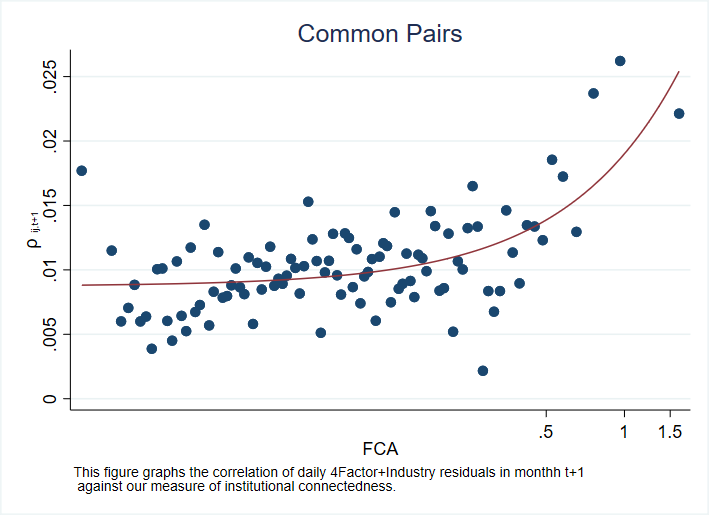
\includegraphics[width=0.7\linewidth]{"Output/mcorr50.eps"} 
		\caption{Future monthly correlation for different level of common ownership at this period }
		\label{mcorr50}
	\end{figure}
	
	We estimate these regressions for each month and report the time-series average as in \cite{FamaMacBeth} to don't have any problem with cross-correlation in the residuals. We then use  \cite{newey1987hypothesis} to calculate standard errors of the Fama-MacBeth that take into account autocorrelation in the time series of cross-sectional estimates for four lags ($ 4(71/100)^{\frac{2}{9}} = 3.71 \sim 4 $).
	
	The estimated results are presented in tables \ref{mresult2part1}
	and \ref{mresult2part2}.
	In the two first columns table \ref{mresult2part1}, we estimate a simplified version of equation \ref{model1} with only common ownership measure ($ MFCAP^*_{i,j}$). In the first column, we estimate the model without control variables. Recall that our control variables are \textit{Same Industry}, \textit{Same Size}, \textit{Same Book to Market}, and \textit{Cross-Ownership}. The \textit{Same Size} and the \textit{Same Book to Market} are normalized to have a standard deviation of one and are transformed so that higher values indicate greater style similarity.  We find that $ MFCAP^*_{i,j}$ is significant with a coefficient of $0.00335$ and a t-statistics of $5.27$ in the presence of control variables. 
	
	
	In Columns 3 and 4 of that table, we use another simplified version of equation \ref{model1}, with only Same Group. The estimated coefficient in this specification, Same Group is highly statistically significant, with a coefficient of   $0.0239$ and a t-statistics of $9.41$. 
	There is a significant difference in the impact of same business groups and the common ownership, according to the results. 
	
	In the fifth specification of table \ref{mresult2part1}, we use both \textit{Same Group}  and $\text{MFCAP}^*_{ij,t}$ as a forecasting variable. In this specification, only  \textit{Same Group} has a significant effect on our estimation. It suggests that pair in the same business group affects more than a higher level of common ownership
	\cite{AntonPolk} study large firms but we do not restrict  our investigation. In the last column of table \ref{mresult2part1}, we control for pairs type (Pairs is large or small if both firms are large or  small . If one firm is large and other is small, we call it hybrid.) Estimation results in table \ref{mresult2part1} shows that for all the pairs \textit{Same Group} significantly increases co-movement.
	
	In Table  \ref{mresult2part2}, we examine effect of common ownership in the business groups. In two first columns, we restrict our investigation to two sub-samples. In the first one, we run our model for the pairs in the same business group and others who do not belong to the same one in the second one. It provides evidence that common ownership only matters for the pairs in the same business groups. 
	
	
	Now for the main analysis, we include the interaction of \textit{Same Group} and $\text{MFCA}^*_{ij,t}$. We include the business group fixed effects to capture the group's characteristics for the last column. In these specifications, ecnomical effect of \textit{Same Group} it is not significant anymore which  cannot reliable due to high corelation of interaction term with \textit{Same Group}($\rho = 0.6$). These results aver that $\text{MFCA}^*_{ij,t}$ has a larger effect for the pairs in the same business group. It puts forward that the \textit{Same Group}  affects co-movement through indirect common ownership, which arises due to the same ultimate owner. 
	
	
	


{\begin{table}[p]
		\centering
		\caption{Connected Co-movement}
		\label{mresult2part1}
		\resizebox{1\textwidth}{!}{
			
				{{
\def\sym#1{\ifmmode^{#1}\else\(^{#1}\)\fi}
\begin{tabular}{l*{6}{c}}
\hline\hline
                    &\multicolumn{6}{c}{Dependent Variable:  Future Pairs's Comovement}                                                                 \\\cmidrule(lr){2-7}
                    &\multicolumn{1}{c}{(1)}         &\multicolumn{1}{c}{(2)}         &\multicolumn{1}{c}{(3)}         &\multicolumn{1}{c}{(4)}         &\multicolumn{1}{c}{(5)}         &\multicolumn{1}{c}{(6)}         \\
\hline
$ \text{MFCAP*} $   &     0.00600\sym{***}&     0.00328\sym{***}&                     &                     &     0.00104         &    0.000929         \\
                    &      (8.10)         &      (4.87)         &                     &                     &      (1.68)         &      (1.53)         \\
[1em]
SameGroup           &                     &                     &      0.0358\sym{***}&      0.0254\sym{***}&      0.0242\sym{***}&      0.0219\sym{***}\\
                    &                     &                     &      (9.99)         &      (8.45)         &      (8.21)         &      (7.02)         \\
[1em]
SameIndustry        &                     &      0.0267\sym{***}&                     &      0.0216\sym{***}&      0.0212\sym{***}&      0.0215\sym{***}\\
                    &                     &      (7.39)         &                     &      (6.81)         &      (6.72)         &      (6.80)         \\
[1em]
SameBM              &                     &      0.0224\sym{***}&                     &      0.0213\sym{***}&      0.0214\sym{***}&      0.0199\sym{***}\\
                    &                     &      (6.41)         &                     &      (6.09)         &      (6.16)         &      (5.77)         \\
[1em]
SameSize            &                     &      0.0123\sym{**} &                     &      0.0143\sym{***}&      0.0138\sym{***}&      0.0254\sym{***}\\
                    &                     &      (3.24)         &                     &      (3.85)         &      (3.71)         &      (5.56)         \\
[1em]
CrossOwnership      &                     &      0.0600\sym{***}&                     &      0.0300\sym{*}  &      0.0316\sym{*}  &      0.0377\sym{**} \\
                    &                     &      (5.50)         &                     &      (2.36)         &      (2.48)         &      (2.93)         \\
[1em]
Constant            &      0.0142\sym{***}&      0.0204\sym{***}&      0.0103\sym{***}&      0.0187\sym{***}&      0.0188\sym{***}&      0.0280\sym{***}\\
                    &     (12.80)         &      (8.91)         &      (9.42)         &      (7.99)         &      (8.04)         &      (9.43)         \\
\hline
PairType Control    &          No         &          No         &          No         &          No         &          No         &         Yes         \\
Observations        &      389591         &      389591         &      389591         &      389591         &      389591         &      389591         \\
\hline\hline  \end{tabular}}
}
			
		}
\end{table}}

{\begin{table}[p]
		\centering
		\caption{Connected Co-movement}
		\label{mresult2part2}
		\resizebox{1\textwidth}{!}{
			
				{{
\def\sym#1{\ifmmode^{#1}\else\(^{#1}\)\fi}
\begin{tabular}{l*{4}{c}}
\hline\hline
                &\multicolumn{4}{c}{Dependent Variable: Future Pairs's co-movement'}        \\\cmidrule(lr){2-5}
                &\multicolumn{1}{c}{(1)}         &\multicolumn{1}{c}{(2)}         &\multicolumn{1}{c}{(3)}         &\multicolumn{1}{c}{(4)}         \\
\hline
$ \text{MFCAP*} $&  0.00944\sym{***}& 0.000397         & 0.000377         &-0.0000113         \\
                &   (7.24)         &   (0.68)         &   (0.65)         &  (-0.02)         \\
[1em]
Same Group      &                  &                  &  0.00624\sym{**} &  0.00549\sym{*}  \\
                &                  &                  &   (2.81)         &   (2.27)         \\
[1em]
 $ (\text{MFCAP}^*) \times {\text{SameGroup} }  $ &                  &                  &  0.00992\sym{***}&   0.0107\sym{***}\\
                &                  &                  &   (6.49)         &   (6.97)         \\
\hline
Observations    &    58337         &  1607659         &  1665996         &  1665996         \\
Sub-sample      &SameGroup         &   Others         &      All         &      All         \\
Group Effect    &       No         &       No         &       No         &      Yes         \\
Controls        &      Yes         &      Yes         &      Yes         &      Yes         \\
$ R^2 $         &   0.0112         & 0.000577         & 0.000898         &  0.00575         \\
\hline\hline
\multicolumn{5}{l}{\footnotesize \textit{t} statistics in parentheses}\\
\multicolumn{5}{l}{\footnotesize \sym{*} \(p<0.05\), \sym{**} \(p<0.01\), \sym{***} \(p<0.001\)}\\
\end{tabular}
}
}
			
		}
\end{table}}


		\FloatBarrier
		
		
		
		\subsection{{High level of common ownership}}
		
			In line with the previous estimations, figure \ref{Qmcorr5lrd} provides that a higher level of common ownership affects more on the firms' co-movement. As shown in table \ref{measureResults}, pairs in the same business group have a higher level of common ownership than others. So, the previous results could be drive from high level of common ownership For detailed analysis, we restrict our sample to the higher level of common ownership, which we define as the pairs with $\text{MFCAP}_{ij,t}$ in the fourth quarter in each period. Figure \ref{Qmcorr5subsample} shows the relation between future co-movement and current measurement of common ownership for that pairs. As you can see in the left panel, in line with the last explanation, common ownership only affects the pairs in the same group, and common ownership without the same group will not affect pairs' co-movement although for a high level of common ownership.
			
			\begin{figure}[htbp]
				\centering  
				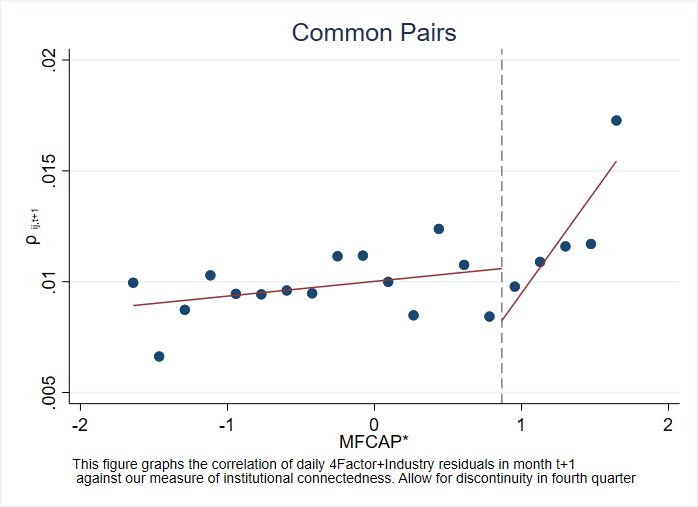
\includegraphics[width=0.6\linewidth]{"Output/Qmcorr5lrd.eps"}
				\caption{Future monthly correlation for different level of common ownership at this period}
				\label{Qmcorr5lrd}
			\end{figure}
			\begin{figure}[htbp]
				\centering  
				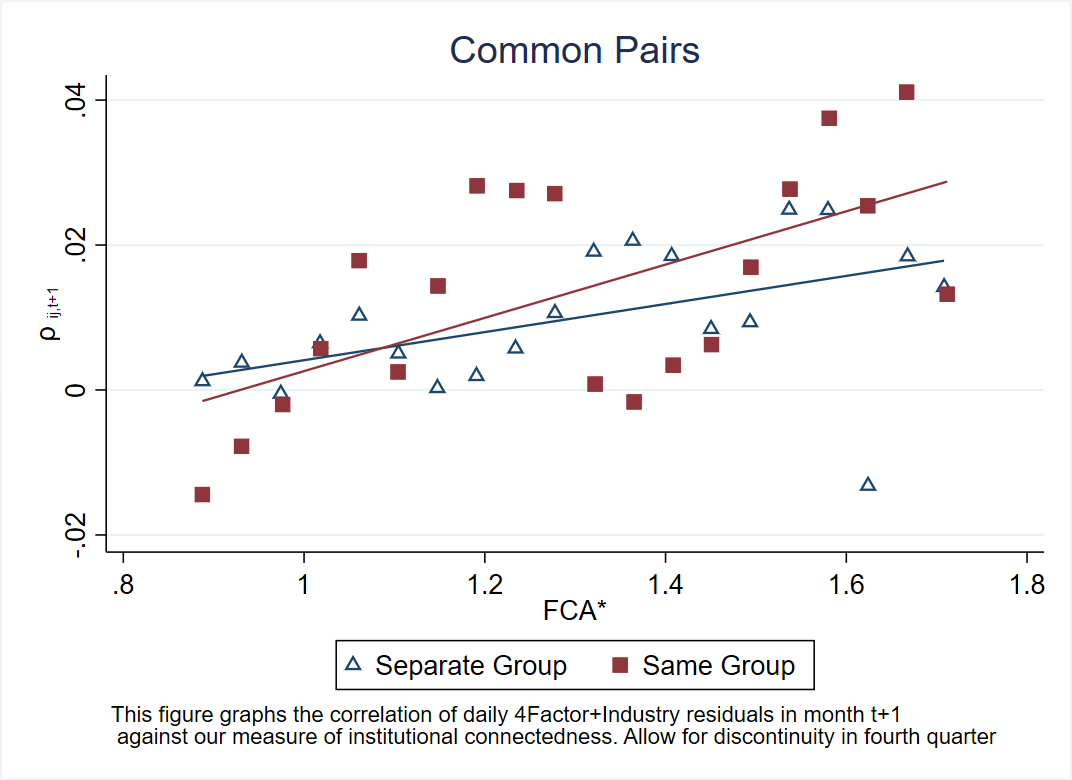
\includegraphics[width=0.45\linewidth]{"Output/Qmcorr5lrdbgsubsample.eps"}
				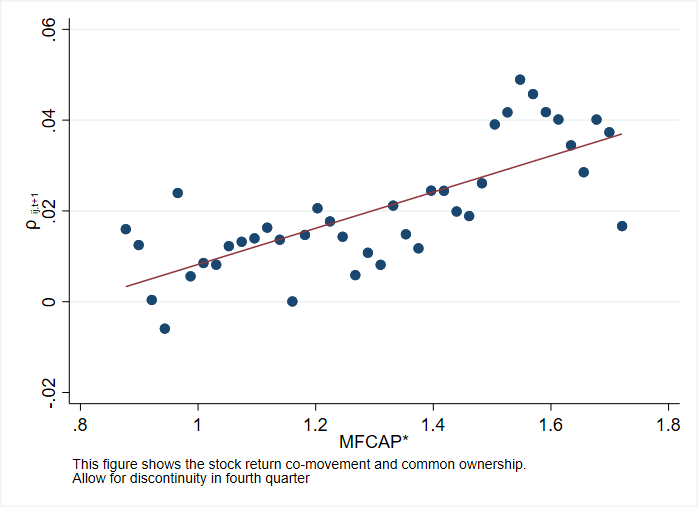
\includegraphics[width=0.45\linewidth]{"Output/Qmcorr5subsample.eps"}
				\caption{Future monthly correlation for different level of common ownership at this period for high level of common ownership}
				\label{Qmcorr5subsample}
			\end{figure}
			
			
			We estimate the equation \ref{model1} with the same methodology in section \ref{Forecasting Co-movement}  for the sub-sample of a high level of common ownership. Table \ref{QTimemresult2subsample} reports estimations results. As expected, firms in the same business group have a high statistical and economically significant effect on forecasting future co-movements. Columns three to seven confirm our prior explanations for the importance of business groups compared to common ownership in pairs with a higher level of common ownership. 
			
			{\begin{table}[htbp]
					\centering
					\caption{\scriptsize Estimation results for high level of common ownership}
					\label{QTimemresult2subsample}
					{
						\resizebox{\textwidth}{!}{
						{
\def\sym#1{\ifmmode^{#1}\else\(^{#1}\)\fi}
\begin{tabular}{l*{7}{c}}
\hline\hline
                &\multicolumn{7}{c}{Dependent Variable:  Future Pairs's Comovement}                                                                  \\\cmidrule(lr){2-8}
                &\multicolumn{1}{c}{(1)}         &\multicolumn{1}{c}{(2)}         &\multicolumn{1}{c}{(3)}         &\multicolumn{1}{c}{(4)}         &\multicolumn{1}{c}{(5)}         &\multicolumn{1}{c}{(6)}         &\multicolumn{1}{c}{(7)}         \\
\hline
SameGroup       &   0.0254\sym{***}&                  &   0.0249\sym{***}&                  &                  &  0.00477         &  0.00252         \\
                &   (8.45)         &                  &   (8.21)         &                  &                  &   (1.32)         &   (0.66)         \\
[1em]
$ (\text{MFCAP} > \text{Larger than 75th Percentile}) $ &                  &  0.00660\sym{***}& 0.000777         &   0.0230\sym{***}& -0.00258\sym{*}  & -0.00157         &-0.000513         \\
                &                  &   (5.48)         &   (0.73)         &   (7.09)         &  (-2.00)         &  (-1.29)         &  (-0.46)         \\
[1em]
 $ (\text{MFCAP} > Q3[\text{MFCAP}]) \times {\text{SameGroup}} $ &                  &                  &                  &                  &                  &   0.0248\sym{***}&   0.0237\sym{***}\\
                &                  &                  &                  &                  &                  &   (7.24)         &   (7.34)         \\
\hline
Sub-sample      &      All         &      All         &      All         &SameGroup         &   Others         &      All         &      All         \\
Controls        &      Yes         &      Yes         &      Yes         &      Yes         &      Yes         &      Yes         &      Yes         \\
Business Group FE&       No         &       No         &       No         &       No         &       No         &       No         &      Yes         \\
Observations    &   389591         &   389591         &   389591         &    47076         &   342515         &   389591         &   389591         \\
\hline\hline
\multicolumn{8}{l}{\footnotesize \textit{t} statistics in parentheses}\\
\multicolumn{8}{l}{\footnotesize \sym{*} \(p<0.05\), \sym{**} \(p<0.01\), \sym{***} \(p<0.001\)}\\
\end{tabular}
}

						}
					}
			\end{table}}
			
			\begin{figure}[htbp]
				\centering  
				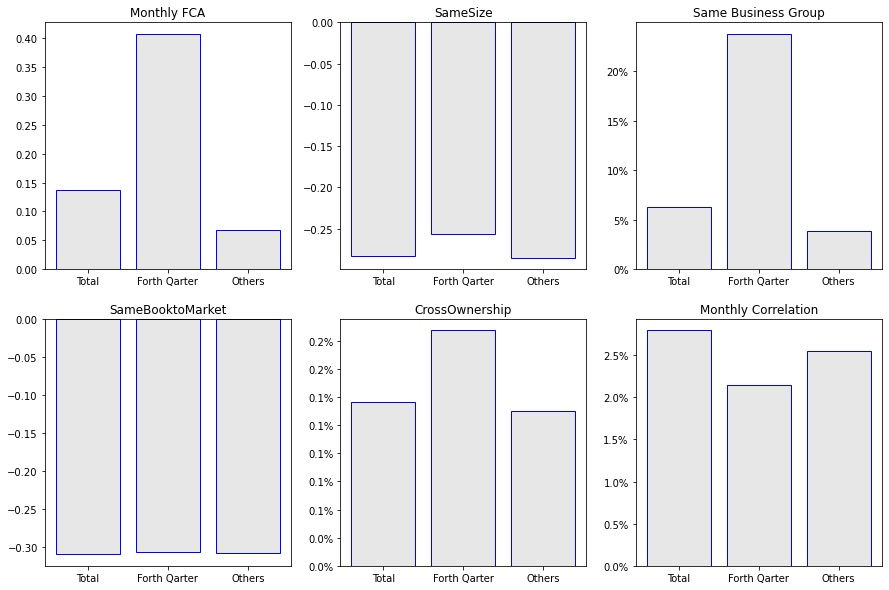
\includegraphics[width=0.75\linewidth]{"Output/QarterSummary.eps"}
				\caption{Pairs' characteristics for the pairs with high level of common ownership}
				\label{QarterSummary}
			\end{figure}
			

				
				
				\FloatBarrier
				
				\subsection{All Pairs}
				
	In the former analyses, we restrict our investigation to firms with at least one common owner. By this analysis, we cannot separate the effect of the business group and common ownership; both of them can affect comovement. Furthermore, this restriction limits our result to commonly held firms, but if belonging to the same business group can increase stocks' comovement, it would affect all the firms in the same business group. 
	So, we extend our investigation by constructing all the pairs in the market to separate the effect of direct common ownership and business group and solve the mentioned problem. 
	
	For this purpose, we include stocks in one pair if they have at least two months in common. By this definition, we do not restrict our investigation to commonly held stocks and set $\text{MFCA}_{ij,t}$ to zero for a pair without any common owner. Controls are defined as before, and we use the same methodology as used for estimating equation \ref{model1}. We estimate equation \ref{model1}. 
	
	Table \ref{AllPairs} reports results of estimations for two models. These results suggest that pairs in the same group co-move more than stocks that are not in the same group. In addition, pairs with common ownership common does not co-move greater than others. In column 3 , we use variables of common ownership and the same business group together. Results supported our previous explanation of table \ref{mresult2part1} that the \textit{Same Group} is critical for forecasting future co-movement, and common ownership does not matter for pairs. Common ownership matters for the pairs in the same business group.
					
					{\begin{table}[htbp]
							%	\centering
							\caption{Non-connected Co-movement}
							\label{AllPairs}
							\resizebox{1\textwidth}{!}{
								
									{	{
\def\sym#1{\ifmmode^{#1}\else\(^{#1}\)\fi}
\begin{tabular}{l*{7}{c}}
\hline\hline
                &\multicolumn{7}{c}{Dependent Variable: Future Pairs' co-movement}                                                                   \\\cmidrule(lr){2-8}
                &\multicolumn{1}{c}{(1)}         &\multicolumn{1}{c}{(2)}         &\multicolumn{1}{c}{(3)}         &\multicolumn{1}{c}{(4)}         &\multicolumn{1}{c}{(5)}         &\multicolumn{1}{c}{(6)}         &\multicolumn{1}{c}{(7)}         \\
\hline
SameGroup       &   0.0156\sym{***}&                  &   0.0158\sym{***}&                  &                  &   0.0138\sym{***}&   0.0131\sym{***}\\
                &   (9.84)         &                  &  (10.22)         &                  &                  &   (8.27)         &   (7.68)         \\
[1em]
$ \text{MFCAP*}  $&                  &-0.0000723         &-0.000277         &  0.00169         &-0.000322\sym{*}  &-0.000390\sym{**} &-0.000427\sym{*}  \\
                &                  &  (-0.44)         &  (-1.80)         &   (1.42)         &  (-2.19)         &  (-2.70)         &  (-2.29)         \\
[1em]
 $ (\text{MFCAP}^*) \times {\text{SameGroup} }  $ &                  &                  &                  &                  &                  &  0.00313\sym{**} &  0.00364\sym{**} \\
                &                  &                  &                  &                  &                  &   (2.80)         &   (3.34)         \\
\hline
Controls        &      Yes         &      Yes         &      Yes         &      Yes         &      Yes         &      Yes         &      Yes         \\
Sub-Sample      &    Total         &    Total         &    Total         &SameGroups         &   Others         &    Total         &    Total         \\
Business Group FE&       No         &       No         &       No         &       No         &       No         &       No         &      Yes         \\
Observations    &  6018646         &  6018646         &  6018646         &   114526         &  5904120         &  6018646         &  6018646         \\
\hline\hline
\multicolumn{8}{l}{\footnotesize \textit{t} statistics in parentheses}\\
\multicolumn{8}{l}{\footnotesize \sym{*} \(p<0.05\), \sym{**} \(p<0.01\), \sym{***} \(p<0.001\)}\\
\end{tabular}
}

									}
							}
					\end{table}}
					
				
					
					
%					
%					In conclusion , these results show that same business group is more important than common ownership. In fact, when we talk about the presence of two stocks in the same business group, we talk about a high level of invisible common ownership between two stocks that we cannot measure that by mutual stockholders.
					
					
					\FloatBarrier

\FloatBarrier
\section{{Evidence for correlated trading} }


	In the previous sections, we have provided evidence consistent with the hypothesis that the presence of firms in the business groups can raise firms' co-movement. Although we don't have definitive insight into the specific channel that business groups can promote commonality, our analysis provides a useful overview.
	We claim that this relationship exists because the business group is an important proxy for the likelihood that trading in these stocks will be correlated. To better understand how the business group can generate co-movement in firms' returns, we now refine our basic analysis to consider other proxy measures for business group trading.
	We employ two proxies for business group trading that are designed to capture different trading motivations: turnover and institutional imbalance. While the first could be due to buying or selling of business groups, the latter reflects buying.
%	We employ one proxy for business group trading that is designed to capture  trading motivations: turnover which could be due to buying or selling of business groups.



\subsection{{Turnover}}


	First, we should show that stocks in groups have a similar daily trading behavior. Accordingly, We use the turnover measure as a daily trading measures. For each firm we run time-series regressions of the firm's daily change in turnover, $ \Delta \text{TurnOver}_{i,t} $, on changes in market turnover,$ \Delta\text{TurnOver}_{Market,t}   $ , changes in the industry and business group portfolio's turnover,$ \Delta\text{TurnOver}_{Ind,t} $ and  $\Delta \text{TurnOver}_{Group,t} $ and  ,as well as control variables.
	We compute the daily change of turnover by this definition $ \Delta \text{TurnOver}_{i,t} = \ln(\frac{\text{TurnOver}_{i,t}}{\text{TurnOver}_{i,t-1}}) $. 
	We estimate the following regression for each stock across trading days in a given year separately, and cross-sectional averages of the estimated coefficients are reported, with t-statistics in parentheses :
	
		\begin{equation*}
	\begin{split}
		\Delta \text{Turnover}_{i,t} =  & \text{	}\alpha + \beta_{Market,t} \Delta \text{Turnover}_{Market,t}  
		+ \beta_{Ind,t} \Delta \text{Turnover}_{Ind,t} \\ & + \beta_{Group,t} \Delta \text{Turnover}_{Group,t} + \delta\text{Controls} + \varepsilon_{i,t}
	\end{split}
\end{equation*}
	  We control for lead and lag changes in the two portfolios and the firm's measures and size. We estimate that model with \cite{FamaMacBeth} method and adjust its standard errors with \cite{newey1987hypothesis} for seven periods.  As shown in Table \ref{turnover}, firms' change in turnover comes from market reaction and group's change (This result is robust to the different methods of weighting for portfolios). This observation shows that firms in one group trade together each day. 
	
	We use our previous methodology to investigate these results. We calculate correlation of $ \Delta \text{TurnOver} $ for founded pairs and examine its relation with our variables. Table \ref{mresult2-turnover} reports the estimation result, which confirms that pairs in the business groups lead to correlated trade. In addition, we study effect of  correlation of $ \Delta \text{TurnOver} $ on co-movement for founded pairs in table \ref{turncomovement}. These results suggest that business groups yield to future co-movement through correlated trading in that month.
  
  
  
  
  
  
{\begin{table}[htbp]
	\centering
	\caption{$\Delta \text{TurnOver}$ of firm and Business group}
	\label{turnover}
	\subcaption{This table reports \cite{FamaMacBeth} estimates of daily change in turnover ($ \Delta \text{TurnOver}_{i,t} = \ln(\frac{\text{TurnOver}_{i,t}}{\text{TurnOver}_{i,t-1}}) $) for all the firms in the market. The independent variables are change in turnover for Market, Insudtry, and Business group for that day. We exclude firm's change from associated groups to prevent spurious correlations. We calculate \cite{newey1987hypothesis} standard errors (seveb lags) of the \cite{FamaMacBeth} estimates that take into account autocorrelation in the cross-sectional slopes. We report the associated t-statistics in parentheses. }
	\resizebox{!}{!}{
		{
\def\sym#1{\ifmmode^{#1}\else\(^{#1}\)\fi}
\begin{tabular}{l*{4}{c}}
\hline\hline
                    &\multicolumn{4}{c}{Dependent Variable: $\Delta \text{TurnOver}\_{i} $ }                 \\\cmidrule(lr){2-5}
                    &\multicolumn{1}{c}{(1)}         &\multicolumn{1}{c}{(2)}         &\multicolumn{1}{c}{(3)}         &\multicolumn{1}{c}{(4)}         \\
\hline
 $ \Delta \text{TurnOver}_{\text{Market}} $ &       0.416\sym{***}&       0.326\sym{***}&       0.252\sym{***}&       0.228\sym{***}\\
                    &     (12.25)         &      (5.35)         &      (6.41)         &      (4.24)         \\
[1em]
 $ \Delta \text{TurnOver}_{\text{Industry-i}} $ &       0.142\sym{***}&       0.213\sym{***}&      0.0335         &       0.167\sym{**} \\
                    &      (3.79)         &      (6.29)         &      (1.34)         &      (2.87)         \\
[1em]
 $ \Delta \text{TurnOver}_{\text{Group,-i}} $ &                     &                     &       0.330\sym{***}&       0.218\sym{***}\\
                    &                     &                     &     (12.74)         &      (3.80)         \\
\hline
Control             &          No         &         Yes         &          No         &         Yes         \\
Observations        &      854662         &      851772         &      333789         &      331263         \\
$ R^2 $             &       0.285         &       0.543         &       0.433         &       0.712         \\
\hline\hline
\multicolumn{5}{l}{\footnotesize \textit{t} statistics in parentheses}\\
\multicolumn{5}{l}{\footnotesize \sym{*} \(p<0.05\), \sym{**} \(p<0.01\), \sym{***} \(p<0.001\)}\\
\end{tabular}
}

	} 
\end{table}}


	\begin{table}[htbp]
		\centering
		\caption{Simultaneous trade and Co-movement}
		\label{mresult2-turnover}
			\subcaption{This table reports \cite{FamaMacBeth} estimates of the pairwise correlation in liquidity for the sample of stocks defined in Table \ref{t2-2}. The independent variables are updated monthly include our measure of institutional connectedness, the number of equal percents held block-holder, $\text{MFCAP}^*_{ij,t}$, and a series of controls at time t. We measure the negative of the absolute value of the difference in size and book-to-market ratio (BE/ME) percentile ranking across the two stocks in the pair (SameSize, and SameBM, respectively). All independent variables, excluding dummy variables, are rank-transformed and normalized to have a unit standard deviation. We calculate \cite{newey1987hypothesis} standard errors (four lags) of the \cite{FamaMacBeth} estimates that take into account autocorrelation in the cross-sectional slopes. We report the associated t-statistics in parentheses. Controls not shown here are reported in the Internet Appendix.}
		\resizebox{\textwidth}{!}{
			\centering
			{
\def\sym#1{\ifmmode^{#1}\else\(^{#1}\)\fi}
\begin{tabular}{l*{7}{c}}
\hline\hline
                    &\multicolumn{7}{c}{Dependent Variable:  Monthly Correlation of Delta turnover}                                                                           \\\cmidrule(lr){2-8}
                    &\multicolumn{1}{c}{(1)}         &\multicolumn{1}{c}{(2)}         &\multicolumn{1}{c}{(3)}         &\multicolumn{1}{c}{(4)}         &\multicolumn{1}{c}{(5)}         &\multicolumn{1}{c}{(6)}         &\multicolumn{1}{c}{(7)}         \\
\hline
SameGroup           &      0.0180\sym{***}&                     &      0.0173\sym{***}&                     &                     &      0.0150\sym{***}&      0.0168\sym{***}\\
                    &      (6.19)         &                     &      (5.53)         &                     &                     &      (4.89)         &      (5.40)         \\
[1em]
$ \text{MFCAP*} $   &                     &     0.00219\sym{**} &    0.000543         &     0.00115         &    0.000372         &    0.000363         &   -0.000413         \\
                    &                     &      (2.84)         &      (0.69)         &      (0.57)         &      (0.41)         &      (0.40)         &     (-0.37)         \\
[1em]
 $ (\text{MFCAP}^*) \times {\text{SameGroup} }  $ &                     &                     &                     &                     &                     &     0.00260         &     0.00296         \\
                    &                     &                     &                     &                     &                     &      (1.03)         &      (1.19)         \\
\hline
Sub-sample          &         All         &         All         &         All         &   SameGroup         &      Others         &         All         &         All         \\
Business Group FE   &          No         &          No         &          No         &          No         &          No         &          No         &         Yes         \\
Observations        &      294864         &      294864         &      294864         &       37076         &      257788         &      294864         &      294864         \\
\hline\hline
\multicolumn{8}{l}{\footnotesize \textit{t} statistics in parentheses}\\
\multicolumn{8}{l}{\footnotesize \sym{*} \(p<0.05\), \sym{**} \(p<0.01\), \sym{***} \(p<0.001\)}\\
\end{tabular}
}

		}
		\label{turncomovement}
		\resizebox{\textwidth}{!}{
			\centering
			{
\def\sym#1{\ifmmode^{#1}\else\(^{#1}\)\fi}
\begin{tabular}{l*{5}{c}}
\hline\hline
                    &\multicolumn{5}{c}{Dependent Variable:  Future Pairs's Comovement}                                           \\\cmidrule(lr){2-6}
                    &\multicolumn{1}{c}{(1)}         &\multicolumn{1}{c}{(2)}         &\multicolumn{1}{c}{(3)}         &\multicolumn{1}{c}{(4)}         &\multicolumn{1}{c}{(5)}         \\
\hline
 $ {\rho(\Delta \text{TurnOver})_{t+1}} $ &      0.0856\sym{***}&      0.0742\sym{***}&       0.152\sym{***}&      0.0611\sym{***}&      0.0743\sym{***}\\
                    &     (14.09)         &     (13.91)         &     (15.57)         &     (11.82)         &     (13.94)         \\
[1em]
 $ {\rho_t} $       &      0.0456\sym{***}&      0.0373\sym{***}&      0.0944\sym{***}&      0.0262\sym{***}&      0.0356\sym{***}\\
                    &     (11.44)         &     (10.58)         &     (13.66)         &      (6.57)         &     (10.71)         \\
\hline
Control             &          No         &         Yes         &         Yes         &         Yes         &         Yes         \\
Sub-sample          &       Total         &       Total         &   SameGroup         &      Others         &       Total         \\
Business Group FE   &          No         &          No         &          No         &          No         &         Yes         \\
Observations        &      338895         &      338895         &       41955         &      296940         &      338895         \\
\hline\hline
\multicolumn{6}{l}{\footnotesize \textit{t} statistics in parentheses}\\
\multicolumn{6}{l}{\footnotesize \sym{*} \(p<0.05\), \sym{**} \(p<0.01\), \sym{***} \(p<0.001\)}\\
\end{tabular}
}

		}
	\end{table}



Furthermore, we have to directly show that firms with a higher level of group turnover have a higher level of co-movement. So, we extract the annual average level of firms and monthly turnover for each month. We assume that the residual of the model belongs to the business groups. We expect firms in the groups to have a lower dispersion in their residuals than firms out of the groups. We calculate firms' residuals by the mentioned hypothesis. Its summary stats is in table \ref{tab:ResidualTrunSummary}. As we expected, residuals in business groups have a lower dispersion than others.


We calculate the standard error of firms' monthly turnover residuals in each business group. Groups' standard errors description is shown in table \ref{tab:ResidualTrunStdSummary} and time series in in figure \ref{fig:GroupedResSTD}. On average, the affiliated firms' standard error is lower than unaffiliated ones. For finding the relation between the standard error of monthly turnover residuals, we define a dummy variable for groups in the low level of standard error, which is lower than the median. For analysis, we restrict our investigations to a subsample of \textit{Same Group} and others and estimate our desired variable.   For further study, we use the interaction of \textit{Same Group} with our dummy variable for the full sample, which confirmed our prior results. As shown in table \ref{Turnovercrosssection}, pairs in the business groups of low dispersion have a higher level of co-movement than other firms.



{			\begin{table}[htbp]
\caption{\hl{heading}}
	\centering
	\subcaption{Panel A: Frims' Monthly residuals' summary statistics}
	\label{tab:ResidualTrunSummary}
	\resizebox{0.8\textwidth}{!}{
		\begin{tabular}{lrrrrrrrr}
\toprule
{} &  Firm\$\textbackslash times\$ Month &   mean &    std &    min &    25\% &    50\% &    75\% &    max \\
Grouped   &                     &        &        &        &        &        &        &        \\
\midrule
Ungrouped &                8050 & -0.001 &  0.822 & -4.789 & -0.509 & -0.016 &  0.504 &  4.407 \\
Grouped   &               18199 &  0.001 &  0.777 & -4.832 & -0.481 & -0.033 &  0.469 &  4.955 \\
\bottomrule
\end{tabular}

	}

			\centering
			\subcaption{Panel B: Gtoups' Monthly residuals' standard erros' summary statistics}
			\label{tab:ResidualTrunStdSummary}
			\resizebox{0.8\textwidth}{!}{
				\begin{tabular}{lrrrrrrrr}
\toprule
{} &  Group \$\textbackslash times\$ Month &   mean &    std &    min &    25\% &    50\% &    75\% &    max \\
Grouped   &                       &        &        &        &        &        &        &        \\
\midrule
Ungrouped &                    72 &  0.776 &  0.108 &  0.516 &  0.694 &  0.774 &  0.840 &  1.140 \\
Grouped   &                  2393 &  0.604 &  0.300 &  0.001 &  0.413 &  0.580 &  0.763 &  2.797 \\
\bottomrule
\end{tabular}

			}
		\end{table}
		
		
		
\begin{figure}[htbp]
	\centering
	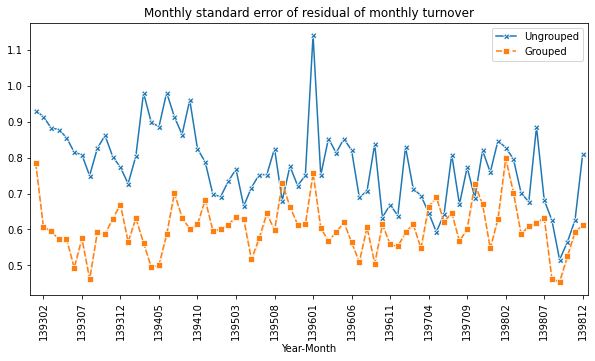
\includegraphics[width=0.85\linewidth]{Output/GroupedResSTD.eps}

	\caption{Average of standard errors in residuals for groups}
	\label{fig:GroupedResSTD}
\end{figure}


		\begin{table}[htbp]
			\centering
			\caption{Estimation results for the relation between low residual std groups and co-movement}
			\label{Turnovercrosssection}			
				\subcaption{\hl{heading}}
			\resizebox{\textwidth}{!}{
				\centering
				{
\def\sym#1{\ifmmode^{#1}\else\(^{#1}\)\fi}
\begin{tabular}{l*{6}{c}}
\hline\hline
                &\multicolumn{6}{c}{Dependent Variable:  Future Pairs's co-movement}                                              \\\cmidrule(lr){2-7}
                &\multicolumn{1}{c}{(1)}         &\multicolumn{1}{c}{(2)}         &\multicolumn{1}{c}{(3)}         &\multicolumn{1}{c}{(4)}         &\multicolumn{1}{c}{(5)}         &\multicolumn{1}{c}{(6)}         \\
\hline
SameGroup       &   0.0208\sym{***}&   0.0210\sym{***}&                  &                  &   0.0137\sym{***}&   0.0113\sym{**} \\
                &   (7.91)         &   (7.77)         &                  &                  &   (3.73)         &   (3.19)         \\
[1em]
LowTurnoverStd  &                  & 0.000929         &   0.0171\sym{***}&-0.000982         & -0.00107         &  0.00279         \\
                &                  &   (0.84)         &   (3.88)         &  (-0.93)         &  (-1.04)         &   (1.39)         \\
[1em]
$ {\text{LowTurnoverStd} } \times {\text{SameGroup} }  $ &                  &                  &                  &                  &   0.0181\sym{***}&   0.0183\sym{***}\\
                &                  &                  &                  &                  &   (3.65)         &   (3.91)         \\
\hline
Sub-sample      &    Total         &    Total         &SameGroup         &   Others         &    Total         &    Total         \\
Business Group FE&       No         &       No         &       No         &       No         &       No         &      Yes         \\
Observations    &   354209         &   354209         &    43274         &   310935         &   354209         &   354209         \\
\hline\hline  \end{tabular}}

			}			
		\end{table}}




\FloatBarrier

%
%
\subsection{{Institutional Imbalance}}

	We should show that stocks in groups that trade together are traded in the same direction. So, for each firm, we calculate daily institutional imbalances, which is the net buying value of institutional investors relative to total traded value on that day ($ \text{InsImb} = \frac{\text{Buy}_{\text{value}} - \text{Sell}_{\text{value}}}{\text{Buy}_{\text{value}} + \text{Sell}_{\text{value}}} $ [\cite{seasholes2007predictable}]).
		We expect that institutional imbalances have a lower variation in groups due to the correlated tradings that the ultimate owner ordered to do. So, we calculate monthly institutional imbalances for firms at the first step. As we expected, firms in the business groups have a lower level of standard error in  imbalances (Table\ref{tab:ImbalanceInsMeanSummary}). Then, we calculate the monthly standard deviation of the group's imbalances and compare them to unaffiliated ones. The standard error is  $12.2\%$ and significantly (with a p-value of 0) lower than ungrouped firms. 
		
	{\begin{table}[htbp]
	\caption{\hl{heading}}
		\centering
		\subcaption{Panel A: Frims' Monthly Imbalances' summary statistics}
			\label{tab:ImbalanceInsMeanSummary}%
		\resizebox{0.75\textwidth}{!}{
			\begin{tabular}{lrrrrrrrr}
\toprule
{} &  Group $\times$ Month &   mean &    std &  min &    25\% &    50\% &    75\% &  max \\
Grouped   &                       &        &        &      &        &        &        &      \\
\midrule
Ungrouped &                 20197 &  0.010 &  0.630 & -1.0 & -0.474 &  0.016 &  0.479 &  1.0 \\
Grouped   &                 12021 & -0.041 &  0.581 & -1.0 & -0.462 & -0.009 &  0.341 &  1.0 \\
\bottomrule
\end{tabular}

		}
	

		\subcaption{Panel B: Gtoups' Monthly Imbalances' standard erros' summary statistics}
				\label{tab:ImbalanceInsStdSummary}%
		\resizebox{0.75\textwidth}{!}{
			\begin{tabular}{lcccccccc}
\toprule
{} &  Group $\times$ Month &   mean &    std &   min &    25\% &    50\% &    75\% &    max \\
Grouped   &                       &        &        &       &        &        &        &        \\
\midrule
Ungrouped &                    72 &  0.624 &  0.054 &  0.48 &  0.601 &  0.631 &  0.655 &  0.735 \\
Grouped   &                  2057 &  0.503 &  0.251 &  0.00 &  0.337 &  0.503 &  0.647 &  1.414 \\
\bottomrule
\end{tabular}

		}
\end{table}}
	\begin{figure}[htbp]
		\centering
		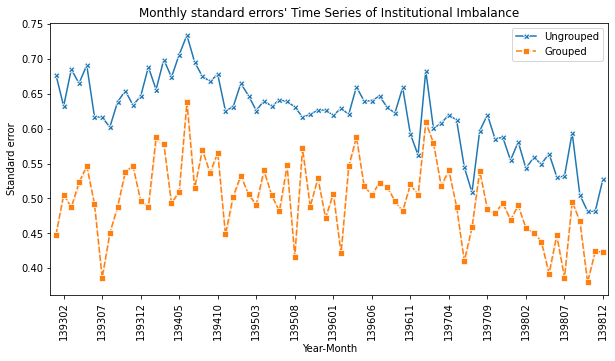
\includegraphics[width=0.85\linewidth]{Output/GroupedInsSTD.eps}
				\caption{Average of standard errors in imbalance for groups}
		\label{fig:GroupedInsSTD}
	\end{figure}
	
	According to the main hypothesis, we need to compare pairs in groups with low standard error and other pairs. For this purpose, we define \textbf{Low Imbalance std} dummy for groups whose average standard errors are lower than half of the sample. So, this dummy is equal to one if at least one pair's firms belong to the low imbalance std business group. We expect pairs in the same business groups with a low standard imbalance error to comove more than others. Table \ref{Imbalance} reports estimation results and confirms that pairs in the low imbalance std comove greater than others. 
	
		{\begin{table}[htbp]
			\centering
			\caption{Estimation results for the relation between low imbalance std groups and co-movement}
			\label{Imbalance}
			\subcaption{\hl{heading}}
			\resizebox{\textwidth}{!}{
				{
\def\sym#1{\ifmmode^{#1}\else\(^{#1}\)\fi}
\begin{tabular}{l*{6}{c}}
\hline\hline
                    &\multicolumn{6}{c}{Dependent Variable:  Future Pairs's Comovement}                                                                 \\\cmidrule(lr){2-7}
                    &\multicolumn{1}{c}{(1)}         &\multicolumn{1}{c}{(2)}         &\multicolumn{1}{c}{(3)}         &\multicolumn{1}{c}{(4)}         &\multicolumn{1}{c}{(5)}         &\multicolumn{1}{c}{(6)}         \\
\hline
SameGroup           &      0.0208\sym{***}&      0.0206\sym{***}&                     &                     &     0.00619         &     0.00630\sym{*}  \\
                    &      (7.91)         &      (7.94)         &                     &                     &      (1.95)         &      (2.04)         \\
[1em]
LowImbalanceStd     &                     &    -0.00144         &      0.0282\sym{***}&    -0.00724\sym{***}&    -0.00610\sym{***}&    -0.00267         \\
                    &                     &     (-1.15)         &      (6.06)         &     (-5.74)         &     (-4.87)         &     (-1.85)         \\
[1em]
 $ \text{LowImbalanceStd} \times {\text{SameGroup} } $ &                     &                     &                     &                     &      0.0358\sym{***}&      0.0325\sym{***}\\
                    &                     &                     &                     &                     &      (8.57)         &      (7.48)         \\
\hline
Sub-sample          &       Total         &       Total         &   SameGroup         &      Others         &       Total         &       Total         \\
Business Group FE   &          No         &          No         &          No         &          No         &          No         &         Yes         \\
Observations        &      354209         &      354209         &       43274         &      310935         &      354209         &      354209         \\
\hline\hline
\multicolumn{7}{l}{\footnotesize \textit{t} statistics in parentheses}\\
\multicolumn{7}{l}{\footnotesize \sym{*} \(p<0.05\), \sym{**} \(p<0.01\), \sym{***} \(p<0.001\)}\\
\end{tabular}
}

			}
	\end{table}}



\FloatBarrier


\section{Conclusion}

 A unique feature of the Iranian stock ownership data is that it is published with daily frequency by the central authority in charge of trading clearing house. This allows us to revisit an important question on the impact of common ownership on stock return comovements. Two firms are defined as commonly owned if they share a direct common owner. Even short of direct common ownership, however, firms can be part of the same business groups, defined as a group of listed firms with interconnected ownership structures controlled by an ultimate owner. Given the prevalent presence of business groups in Iran's public sector, we focus on both direct and indirect common ownership. Direct common ownership is proxied by a modified version of the measure introduced in \cite{AntonPolk}. We use affiliation with the same busness group as a proxy for indirect common ownership. The average common ownership measure is five times larger for firms in the same business group. 
 
We find that business group affiliation is positively associated with higher stock return comovement. Moreover, among firm pairs that belong to the same business groups, those with higher direct common ownership experience higher levels of return comovement. Additional analyses suggest simultaneous trades in the same direction among firms affiliated with the same business groups explains higher return comovements among those stocks, and that direct common ownership likely facilitate simultaneous trading.
\improvement{Is there any implications?}

	


\newpage
	{
	\footnotesize
		\bibliographystyle{apalike}
		\bibliography{../Report/Ref}
	}






%
\begin{appendices}

	
	
	\section{{Overview of Business Groups in Tehran Stock Exchange}} \label{BGDef}
	There is no difference between emerging markets (such as  Chile, India, Indonesia, South Korea, Pakistan, and many more) and developed ones (like Italy and Sweden); business groups present everywhere. However, group-affiliated firms are relatively large and economically important in emerging markets. 
	These groups principally consist of legally independent firms grouped by persistent formal (e.g., equity) and informal (e.g., family) links.(\cite{khanna2007business}) 
	There is a complex ownership network in TSE as an emerging market. 
	This complicated ownership creates a vast number of business groups in which an ultimate owner controls them through a multi-layer of ownership. (\cite{FirmInterlock})
	
	
	
	
	The reason for many of these business groups back to the 1979 Iran revolution. After the revolution, due to social sentiment, critical sectors of the economy nationalized, and their ownership transferred to the government or other pseudo-government foundations. Also,
	some other groups of firms in heavy industries were established and controlled by the Industrial Development and Renovation Organization (IDRO) during the 1960s and 1970s. (IDRO was a state-owned holding company for investing in capital-intensive industries) 
	
	The business groups are formed from mentioned ancestors due to two related forces; A multi-phased privatization by the state and the development of the domestic stock market. In the first wave of privatization, more than 300 companies were fully or partially privatized. In the second one, approximately  \$150 billion ownership of State-Owned Enterprises (SOEs) and assets were transferred.  
	Pension funds, military institutions, cultural and religious foundations, and revolutionary foundations (pseudo-government groups) primary customers in the second wave of privatization. These waves of privatization transferred control of hundreds of SOEs to semi-governmental groups and were the main driver of the formation of business groups in Iran. In addition, the developing stock market from the early 2000s intensifies this effect. The government tried to develop the stock market as a tool for better privatization. 
	(\cite{Aliabadi2022})
	
	In conclusion, the multiple waves of privatization with the development of the stock market changed ownership structure in pre-revolutionary holding companies and post-revolutionary foundations and create large business groups that govern primary  industries.
	
	

%			\begin{figure}[htbp]
%				\caption{}
%				\label{sameIndustryinBG}
%				\centering
%				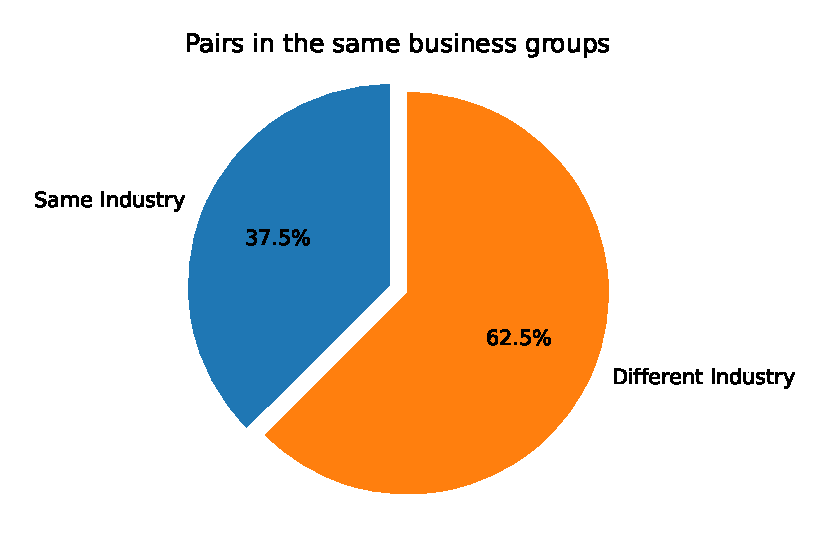
\includegraphics[width=0.48\linewidth]{Output/sameIndustryinBG.eps}
%				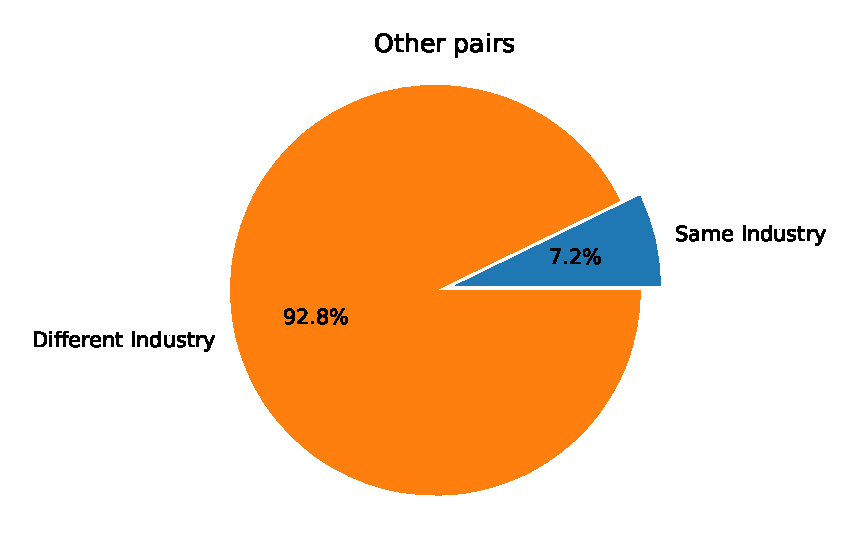
\includegraphics[width=0.48\linewidth]{Output/sameIndustryNoinBG.eps}
%			\end{figure}
%		
%			\begin{figure}[htbp]
%				\caption{}
%				\label{BGSummary}
%				\centering
%				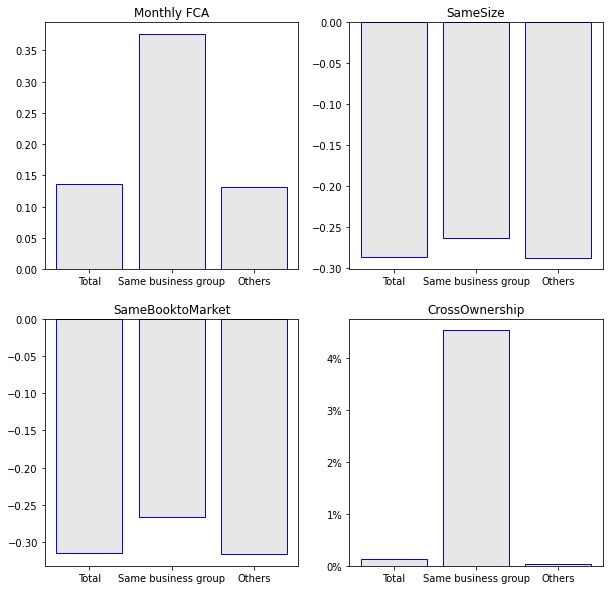
\includegraphics[width=0.85\linewidth]{Output/BGSummary.eps}
%			\end{figure}
%	
	
	
	\FloatBarrier


	\section{{Modified Anton's measure}}
	\label{ModifiedMeasure}
We reformulate mentioned Anton's measure in table \ref{maasurmentsSummary}. This factor measure common ownership as the total value of
stock held by the F common-holders of the two stocks, scaled by the total market capitalization of the two stocks

		\begin{equation}
			\text{Overlap}_{Sum}(i, j) = \frac{\sum_{f = 1}^{F} (S^f_{i,t}P_{i,t}+S^f_{j,t}P_{j,t})}{S_{i,t}P{i,t} + S_{j,t}P{j,t}}
			\label{Sum}
		\end{equation}
where $ S^f_{i,t}$ is the number of shares held by owner f
at time t trading at price $ P{i,t} $ with total shares outstanding of $ S_{i,t} $, and similarly for stock j. 
As shown in equation \ref{Sum}, this measure neglects different distributions of common owners and represents the percent of joint-held market capitalization from the total market capitalization of the two stocks.

We re-weight this formula to capture the difference between ownership distributions. Our proposed measures are shown in equations \ref{sqrt} and \ref{Quadratic}, where all variables are as the same as Anton's measure. Both modified measures represent the number of block-holders with equal-percent ownership. In other words, if for a pair of stocks with n mutual owners, all owners have even shares of each firm's market cap, the proposed indices equals to the number of holders.\footnote{Each holder owns $ 1/n $ of each firm ,firm's market cap is $ \alpha_1 $ and $ \alpha_2 $, so for each holder of firms we have $ S^f_{i,t}P_{i,t} = \alpha_i/n $\\
		$
		[  \frac{\sum_{f=1}^{n} \sqrt{\alpha_1/n}+\sum_{f=1}^{n} \sqrt{\alpha_2/n}}{\sqrt{\alpha_1} + \sqrt{\alpha_2}}]^2 
		= [\frac{\sqrt{n}(\sqrt{\alpha_1} +\sqrt{\alpha_2 })}{\sqrt{\alpha_1} + \sqrt{\alpha_2}}]^2 = n $
		\\
		$
		[\frac{\sum_{f=1}^{n} {(\alpha_1/n)^2}+\sum_{f=1}^{n} {(\alpha_2/n)^2}}{\alpha_1^2 +{\alpha_2}^2}]^{-1} = [\frac{{\alpha_1^2 + \alpha_2^2 }}{n(\alpha_1^2 + \alpha_2^2)}]^{-1} = n
		$} There are some numeric examples for a better comparison. 

		\begin{equation}
			\text{Overlap}_{Sqrt}(i, j) =  [\frac{\sum_{f =1}^{F}(\sqrt{S^f_{i,t}P_{i,t}}+\sqrt{S^f_{j,t}P_{j,t}})}{\sqrt{S_{i,t}P{i,t}} + \sqrt{S_{j,t}P{j,t}}}]^2 
			\label{sqrt}
		\end{equation}
		
		\begin{equation}
			\text{Overlap}_{Quadratic}(i, j) =  [{\frac{\sum_{f = 1}^{F}[(S^f_{i,t}P_{i,t})^2+(S^f_{j,t}P_{j,t})^2]}{(S_{i,t}P{i,t})^2 + (S_{j,t}P{j,t})^2}}]^{-1}
			\label{Quadratic}
		\end{equation}


For the first example, two firms (X and Y) have one common owner who has $ \alpha $ and $ \beta $ from each market capitalization, respectively (illustrated in figure \ref{gExample1}).  
For better illustration, assume that the sum of holders' ownership equals to 100 percent ($ \alpha + \beta  = 100$), and two firms' market caps have equal amounts. 
				\begin{figure}[htbp]
					\centering
					\caption{{ Numeric example 1} }
					\label{gExample1}
					\resizebox{0.65\textwidth}{!}{
										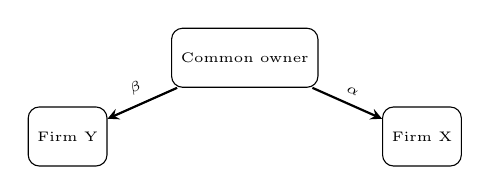
\begin{tikzpicture}[node distance=1cm]
											
											\node (Firm) [startstop3] {\tiny Firm X};
											\node (Firm2) [startstop3,right of = Firm  , xshift=-5.5cm ] {\tiny Firm Y};
											\node (Owner) [startstop3,right of = Firm , yshift=1cm , xshift=-3.25cm ] {\tiny Common owner };
											
											
											\draw[arrow] (Owner) -- node[sloped, anchor=center, above] {\tiny $ \alpha $} (Firm) ;
											
											\draw[arrow] (Owner) -- node[sloped, anchor=center, above] {\tiny $ \beta $} (Firm2) ;
											%
											%\node() at (3,0)
											%    {$ \alpha + \beta = 100 $}; 
										\end{tikzpicture}
									}
									\end{figure}		
We  calculate common ownership measures based on equations \ref{Sum} (Sum), \ref{sqrt} (SQRT), and \ref{Quadratic} (Quadratic) for different ownership distributions. Figure \ref{example1Results}  reports calculations results. As we expected, Anton's measure is constant at a fixed level of aggregated common ownership, but SQRT and Quadratic vary from concentrated to dispersed ownership.  Concentrated ownership (50-50) has a greater common ownership measure than dispersed (10-90).
				
				\begin{figure}[htbp]
					\caption{ {Comparison of three measures for common ownership}}
					\label{example1Results}
					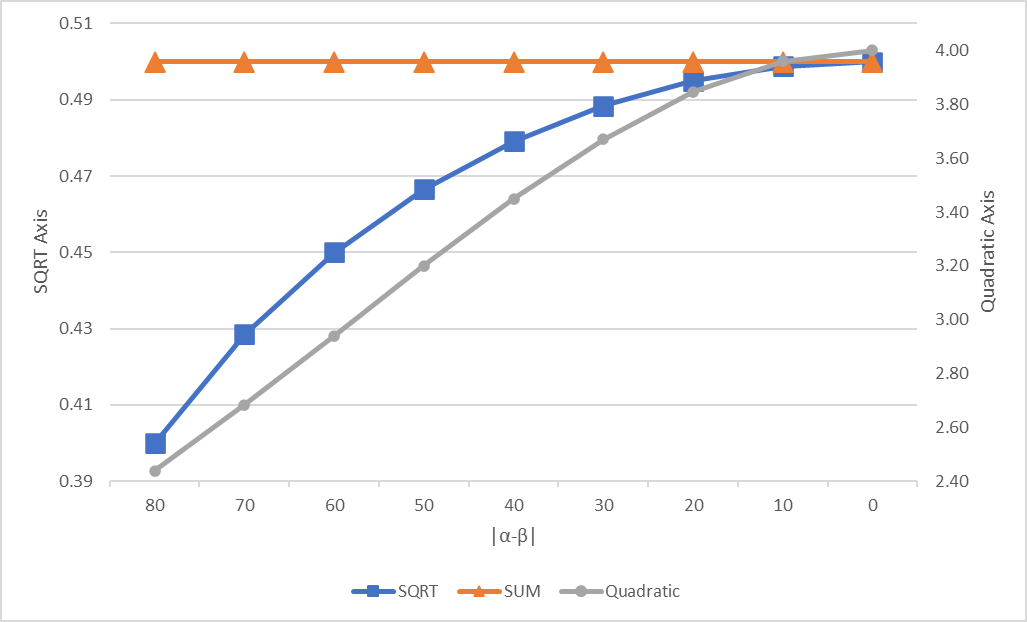
\includegraphics[width=0.47\linewidth]{Elements/1.png}
					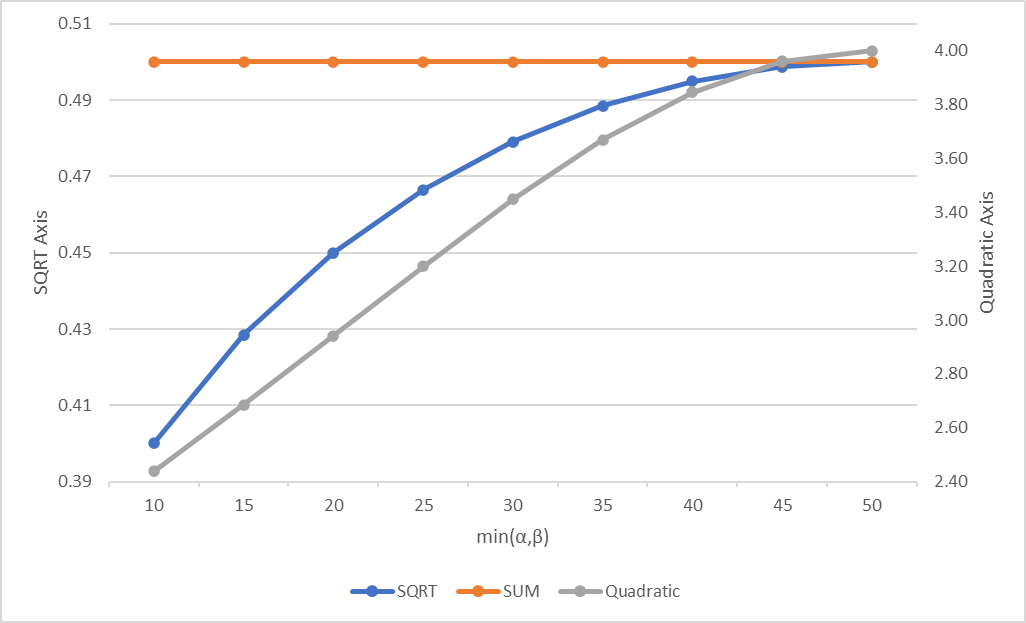
\includegraphics[width=0.47\linewidth]{Elements/2.png}
				\end{figure}

For the second example, assume that there are three common owners for the two mentioned firms. First holder's ownership from firm X and Y are respectively $\alpha_1$ and $\beta_1$. It is similar for other holders (illustrated in figure \ref{gExample2}). As before, the firm's market cap is equal. We calculate measures for concentrated or disparate ownerships, and ownerships that are less than the sum of the market caps. Table \ref{Example2} reports calculation results. For ownerships that consist of total market cap,  results are consistent with the first example. Although, when total ownership decreases, the Quadratic measure denotes unrealistic numbers. We conclude that our Quadratic measure is not suitable for lower levels of common ownership.
				
				\begin{figure}[htbp]  \centering
					\caption{ Numeric example 2}
					\label{gExample2}
					\centering
					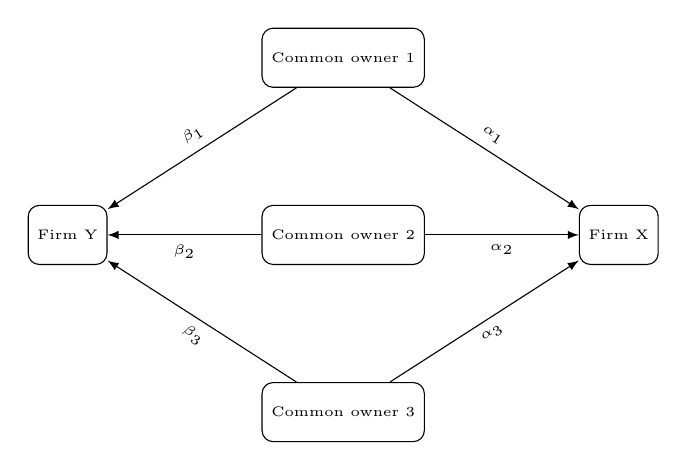
\begin{tikzpicture}[node distance=1cm]
						
						
						\node (Firm) [startstop3] {\tiny Firm X};
						\node (Firm2) [startstop3,right of = Firm , yshift=0cm , xshift=-8cm ] {\tiny Firm Y};
						
						\node (Owner) [startstop3,above of = Firm , yshift=1.25cm , xshift=-3.5cm ] {\tiny Common owner 1 };
						
						
						\node (Owner2) [startstop3,right of = Firm , yshift= 0 , xshift=-4.5cm ] {\tiny Common owner 2 };
						
						\node (Owner3) [startstop3,below of = Firm , yshift=-1.25cm , xshift=-3.5cm ] {\tiny Common owner 3 };
						
						
						
						
						
						\draw [-latex] (Owner) to [bend right =0]  node[sloped, anchor=center, above] {\tiny $ \beta_1 $} (Firm2);
						
						\draw [-latex] (Owner) to [bend left =0]  node[sloped, anchor=center, above] {\tiny $ \alpha_1 $} (Firm);
						
						
						
						\draw [-latex] (Owner2) to [bend right =0]  node[sloped, anchor=center, below] {\tiny $ \beta_2 $} (Firm2);
						
						\draw [-latex] (Owner2) to [bend left =0]  node[sloped, anchor=center, below] {\tiny $ \alpha_2 $} (Firm);
						
						
						
						\draw [-latex] (Owner3) to [bend left =0]  node[sloped, anchor=center, below] {\tiny$ \beta_3 $} (Firm2);
						
						\draw [-latex] (Owner3) to [bend right =0]  node[sloped, anchor=center, below] {\tiny $ \alpha_3 $} (Firm);
						
						
						
					\end{tikzpicture}
				\end{figure}
			{\begin{table}[htbp]
							\centering
							\caption{ text}
							\label{Example2}
							\resizebox{1\textwidth}{!}
							{
								    \begin{tabular}{cccccccc}
    \hline\hline
        Ownership  & Type I & Type II & Type III & Type IV & Type V & Type VI & Type VII \\
          \hline
    $ \alpha_1 $    & 1/3 &20      &  10   & 20    & 10    & 5     & 1  \\
    $ \beta_1 $    & 1/3  & 10    & 10   & 20    & 10    & 5     & 1  \\
    $ \alpha_2 $    & 1/3  & 10    & 80    & 20    & 10    & 5     & 1 \\
    $ \beta_2 $    & 1/3  & 20    & 80    & 20    & 10    & 5     & 1  \\
    $ \alpha_3 $    & 1/3  & 70    & 10    & 20    & 10    & 5     & 1 \\
    $ \beta_3 $    & 1/3  & 70    & 10   & 20    & 10    & 5     & 1  \\
    \hline
    SQRT  & 3     &  2.56  & 2.33 & 1.8   & 0.9   & 0.45  & 0.09 \\
    SUM   & 1     & 1     & 1     & 0.6   & 0.3   & 0.15  & 0.03 \\
    Quadratic & 3     & 1.85  & 1.52  & 8.33  & 33.33 & 133.33 & 3333.33 \\
 
    \hline\hline
    \end{tabular}%
							}
					\end{table}}
				

A fundamental assumption in previous examples, is the equality of firms' market cap. In the last example, we relax this assumption. Table \ref{marketcap} reports calculated measures for fixed total ownership on different relative market cap ratios. We extend our analysis to higher market cap ratios and report our results in figures \ref{sqrtMarket} and \ref{sumMarket}. In this setting, the SQRT measure has a better variation compared to Anton's measure. 

				
	
					\begin{figure}[htbp]
							\centering
							\caption{ SQRT measure for fixed aggregate ownership on different relative market cap ratios}
							\label{sqrtMarket}
							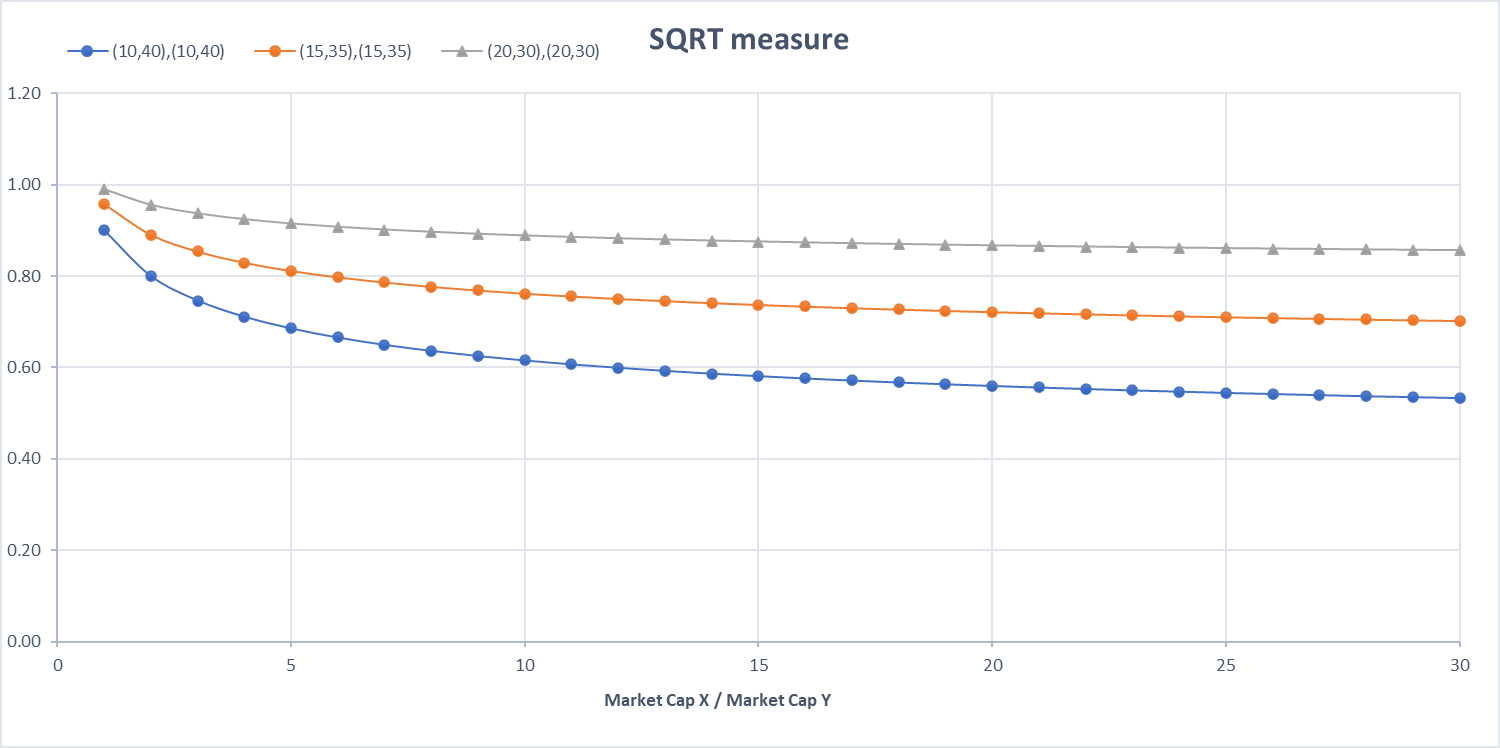
\includegraphics[width=0.85\linewidth]{Elements/3.png}
						\end{figure}
						\begin{figure}[htbp]
							\centering
							\caption{ Sum measure for fixed aggregate ownership on different relative market cap ratios}
							\label{sumMarket}
							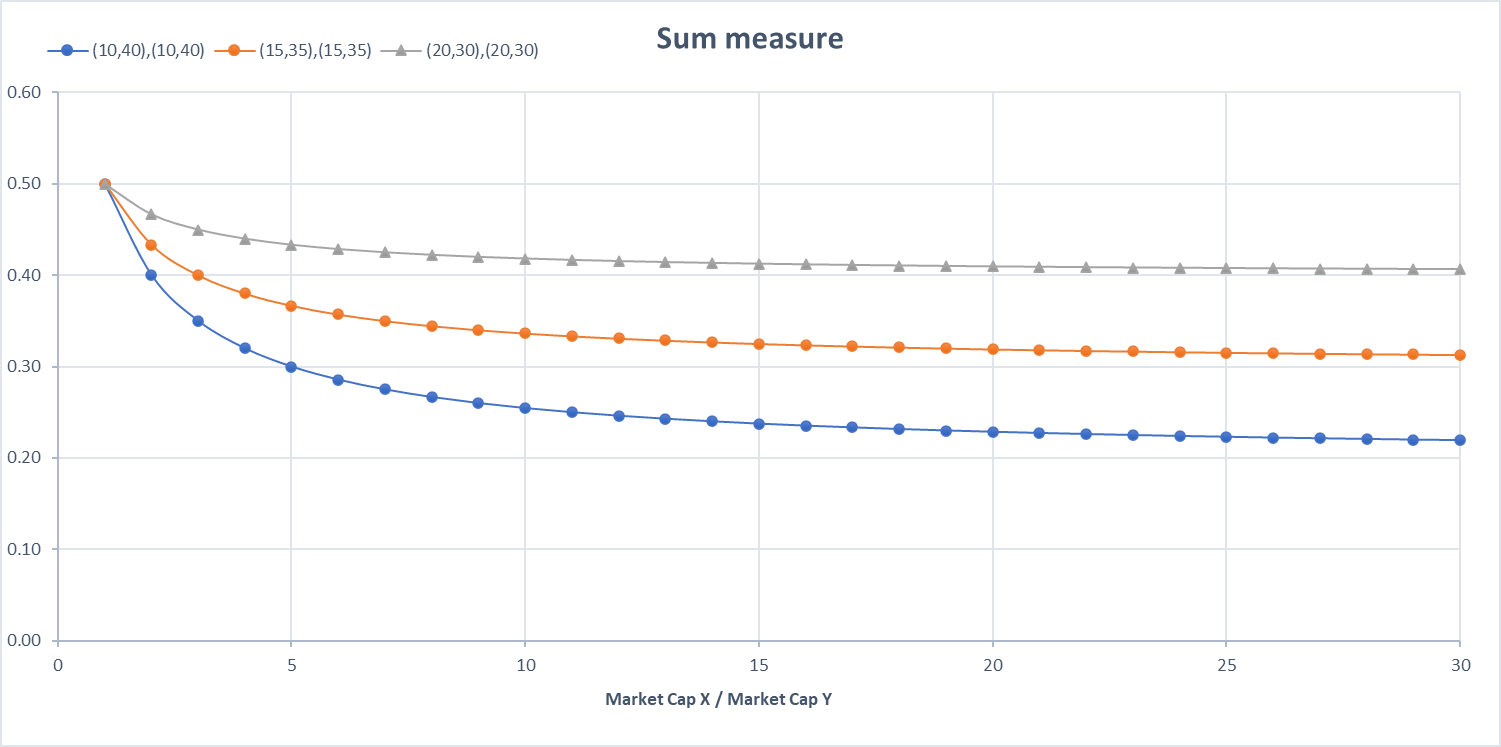
\includegraphics[width=0.85\linewidth]{Elements/4.png}
					\end{figure}
				\begin{table}[htbp]
							\centering
							\caption{text }
							\label{marketcap}
							\resizebox{0.9\textwidth}{!}
							{
								          \scriptsize
    \begin{tabular}{ccccccc}
    \hline\hline
  & \multicolumn{6}{c}{\tiny($ \alpha_1 $,$ \beta_1 $),($ \alpha_2 $,$ \beta_2 $) }\\ \cmidrule(lr){2-7}
               & \multicolumn{2}{c}{\tiny(10,40),(10,40)} & \multicolumn{2}{c}{\tiny(15,35),(15,35)} & \multicolumn{2}{c}{\tiny(20,30),(20,30)} \\ \cmidrule(lr){2-3}\cmidrule(lr){4-5}\cmidrule(lr){6-7}
    \tiny $ \frac{\text{MarketCap}_x}{\text{MarketCap}_y} $     &\tiny SQRT  & \tiny SUM   &\tiny SQRT  &\tiny SUM   &\tiny SQRT  &\tiny SUM \\ 
     \hline\addlinespace

         1     & 0.90  & 0.50  & 0.96  & 0.50  & 0.99  & 0.50 \\
         2     & 0.80  & 0.40  & 0.89  & 0.43  & 0.96  & 0.47 \\
         3     & 0.75  & 0.35  & 0.85  & 0.40  & 0.94  & 0.45 \\
         4     & 0.71  & 0.32  & 0.83  & 0.38  & 0.92  & 0.44 \\
         5     & 0.69  & 0.30  & 0.81  & 0.37  & 0.91  & 0.43 \\
         6     & 0.67  & 0.29  & 0.80  & 0.36  & 0.91  & 0.43 \\
         7     & 0.65  & 0.28  & 0.79  & 0.35  & 0.90  & 0.43 \\
         8     & 0.64  & 0.27  & 0.78  & 0.34  & 0.90  & 0.42 \\
         9     & 0.63  & 0.26  & 0.77  & 0.34  & 0.89  & 0.42 \\
         10    & 0.62  & 0.25  & 0.76  & 0.34  & 0.89  & 0.42 \\
     
    \hline\hline
    \end{tabular}
							}
					\end{table}


In conclusion, We use the SQRT measure for our main study. This measure has an acceptable variation within different distributions and relative market caps. Also, it has a fair value at a lower level of total common ownership. 
	As it is presented in the table \ref{mresult2Polk}, the obtained results are robust to different measurements of common ownership.
%	\subsection{Common Ownership measure}

	{\begin{table}[htbp]
			%	\centering
			\caption{Connected Co-movement}
			\label{mresult2Polk}
			\resizebox{1\textwidth}{!}{
			{{
\def\sym#1{\ifmmode^{#1}\else\(^{#1}\)\fi}
\begin{tabular}{l*{8}{c}}
\hline\hline
                &\multicolumn{8}{c}{Dependent Variable: Future Monthly Correlation of 4F+Industry Residuals}                                                            \\\cmidrule(lr){2-9}
                &\multicolumn{1}{c}{(1)}         &\multicolumn{1}{c}{(2)}         &\multicolumn{1}{c}{(3)}         &\multicolumn{1}{c}{(4)}         &\multicolumn{1}{c}{(5)}         &\multicolumn{1}{c}{(6)}         &\multicolumn{1}{c}{(7)}         &\multicolumn{1}{c}{(8)}         \\
\hline
Common Ownership Measure&  0.00370\sym{***}&  0.00325\sym{***}&  0.00155\sym{*}  &  0.00109         & 0.000333         &-0.000105         & 0.000550         & 0.000283         \\
                &   (5.58)         &   (4.97)         &   (2.61)         &   (1.84)         &   (0.54)         &  (-0.17)         &   (1.07)         &   (0.58)         \\
[1em]
SameGroup       &                  &                  &   0.0229\sym{***}&   0.0234\sym{***}&   0.0100\sym{**} &   0.0103\sym{**} &  0.00626         &  0.00668         \\
                &                  &                  &   (7.89)         &   (7.93)         &   (3.26)         &   (3.17)         &   (1.79)         &   (1.79)         \\
[1em]
 $ \text{\small Common Ownership Measure} \times {\text{SameGroup} }$ &                  &                  &                  &                  &   0.0134\sym{***}&   0.0135\sym{***}&   0.0127\sym{***}&   0.0126\sym{***}\\
                &                  &                  &                  &                  &   (9.47)         &  (10.65)         &   (9.23)         &   (9.71)         \\
\hline
Observations    &   398818         &   398818         &   398818         &   398818         &   398818         &   398818         &   398818         &   398818         \\
Group FE        &       No         &       No         &       No         &       No         &       No         &       No         &      Yes         &      Yes         \\
Measurement     &      Sum         &      Sum         &      Sum         &      Sum         &      Sum         &     SQRT         &      Sum         &     SQRT         \\
$ R^2 $         &  0.00433         &  0.00427         &  0.00518         &  0.00515         &  0.00554         &  0.00551         &   0.0182         &   0.0182         \\
\hline\hline
\multicolumn{9}{l}{\footnotesize \textit{t} statistics in parentheses}\\
\multicolumn{9}{l}{\footnotesize \sym{*} \(p<0.05\), \sym{**} \(p<0.01\), \sym{***} \(p<0.001\)}\\
\end{tabular}
}
}
			}
	\end{table}}
	
	\FloatBarrier
	

\end{appendices}


\end{document}